\title{Supporting Materials for\\
	``State-Building through Public Land Disposal? An Application of Matrix Completion Methods for Counterfactual Prediction''}

\date{}

%%%%%%%%%%%%%%%%%%%%%%%%%%%%%%%%%%%%%%%%%%%%%%%%%%
% Set document class
\documentclass[12pt]{article}

% Define packages
\usepackage{hyperref, url} 
\usepackage{graphicx,amsfonts,psfrag,layout,subcaption,array,longtable,lscape,booktabs,dcolumn,amsmath,amssymb,amssymb,amsthm,setspace,epigraph,chronology,color,colortbl,caption,wasysym,diagbox,natbib,colortbl}
\usepackage[]{graphicx}\usepackage[]{color}
\usepackage[page]{appendix}
\usepackage[section]{placeins}
\usepackage[linewidth=1pt]{mdframed}
\usepackage[margin={1in}]{geometry} %1 inch margins

% Reference labels in the online appendix
\usepackage{xr}
\externaldocument{land-reform}

% Footnotes stick at the bottom
\usepackage[bottom]{footmisc}

% New footnote characters
\usepackage{footmisc}
\DefineFNsymbols{mySymbols}{{\ensuremath\dagger}{\ensuremath\ddagger}\S\P
   *{**}{\ensuremath{\dagger\dagger}}{\ensuremath{\ddagger\ddagger}}}
\setfnsymbol{mySymbols}

% New tabular environment
\usepackage{tabularx}
\newcolumntype{Y}{>{\raggedleft\arraybackslash}X}% raggedleft column X

% Define appendix 
\renewcommand*\appendixpagename{Appendix}
\renewcommand*\appendixtocname{Appendix}

% Position floats
\renewcommand{\textfraction}{0.05}
\renewcommand{\topfraction}{0.95}
\renewcommand{\bottomfraction}{0.95}
\renewcommand{\floatpagefraction}{0.35}
\setcounter{totalnumber}{5}

% Colors for highlighting tables
\definecolor{Gray}{gray}{0.9}

% Different font in captions
\newcommand{\captionfonts}{\scriptsize}

\makeatletter  % Allow the use of @ in command names
\long\def\@makecaption#1#2{%
  \vskip\abovecaptionskip
  \sbox\@tempboxa{{\captionfonts #1: #2}}%
  \ifdim \wd\@tempboxa >\hsize
    {\captionfonts #1: #2\par}
  \else
    \hbox to\hsize{\hfil\box\@tempboxa\hfil}%
  \fi
  \vskip\belowcaptionskip}
%\makeatother   % Cancel the effect of \makeatletter
 
% Set Spacing
%\singlespacing
%\doublespacing

% Number assumptions
\newtheorem*{assumption*}{\assumptionnumber}
\providecommand{\assumptionnumber}{}
\makeatletter
\newenvironment{assumption}[2]
 {%
  \renewcommand{\assumptionnumber}{Assumption #1}%
  \begin{assumption*}%
  \protected@edef\@currentlabel{#1}%
 }
 {%
  \end{assumption*}
 }
\makeatother

% Macros
\newcommand{\Adv}{{\mathbf{Adv}}}       
\newcommand{\prp}{{\mathrm{prp}}}                  % How to define new commands 
\newcommand{\calK}{{\cal K}}
\newcommand{\outputs}{{\Rightarrow}}                
\newcommand{\getsr}{{\:\stackrel{{\scriptscriptstyle\hspace{0.2em}\$}}{\leftarrow}\:}}
\newcommand{\andthen}{{\::\;\;}}    %  \: \; for thinspace, medspace, thickspace
\newcommand{\Rand}[1]{{\mathrm{Rand}[{#1}]}}       % A command with one argument
\newcommand{\Perm}[1]{{\mathrm{Perm}[{#1}]}}       
\newcommand{\Randd}[2]{{\mathrm{Rand}[{#1},{#2}]}} % and with two arguments
\newcommand{\E}{\mathrm{E}}
\newcommand{\Var}{\mathrm{Var}}
\newcommand{\Cov}{\mathrm{Cov}}
\DeclareMathOperator*{\plim}{plim}
\newcommand\independent{\protect\mathpalette{\protect\independenT}{\perp}}
\def\independenT#1#2{\mathrel{\rlap{$#1#2$}\mkern2mu{#1#2}}}
\newcommand{\possessivecite}[1]{\citeauthor{#1}'s [\citeyear{#1}]} 

\renewcommand*\contentsname{Table of contents}

%%%%%%%%%%%%%%%%%%%%%%%%%%%%%%%%%%%%%%%%%%%%%%%%%%%%%%%%%%%%%%%%%%%%%%%%%%%%

\begin{document}

\begin{singlespacing}
\maketitle \thispagestyle{empty}
\tableofcontents \thispagestyle{empty}
\end{singlespacing}

\pagenumbering{roman}% Roman-numbered pages (start from i)

\pagebreak
\pagenumbering{arabic}% Arabic-numbered pages (start from 1)

\section{Exploratory data analysis} \label{eda}

\begin{table}[htbp]
	\captionsetup{font=normalsize}
	\caption{Definitions and data sources of variables.\label{dv-table}}
	\begin{center}
	\scalebox{.6}{	\begin{tabular}{@{}l|llll@{}}
\hline\hline
\textbf{Theme}                     & \textbf{Variable}                                           & \textbf{Coverage}                     & \textbf{Definition}     & \textbf{Source}                            											     \\
\hline
                                   &                                                             &                                    &             &                                                                                                                                                                                                   \\                                                            
\textbf{Farms} 	      & Farm size          & 1860                        & Log average farm size           & \citet{haines2010}                                                                                                                                                    \\                               
%	      & Farm tenancy           & 1880-1950 (decennial)                        & Share of farms operated by tenants          & Ibid.                                                                                                                                                    \\
%                                   &                                                             &                                    &             &                     \\
%	   & Farm wages              & 1870, 1900         &  Log annual agricultural wages paid with board as a share of adult male population         & Ibid.       \\
                                     &                                                             &                            &               &            \\     
		&  Farm value                                               &  1850,1860                           & Log average value of farmland and buildings per acre (\$)          & \citet{haines2010}             \\    
                                   &                                                             &                                 &             &                                                                                                                                                                                                   \\                                           
% &  Farm output                                               & 1870-1900 (decennial)                        & Log value of all farm output as a share of the total number of farms          & Ibid.              \\
%                                   &                                                             &                                    &             &                                                                                                                                                                                                   \\              
			      & Land inequality                                               & Ibid.                        & Gini coefficient based on distribution of farm sizes,     & Ibid.   \\
  				&                  &          &  adjusted for the share of propertyless farmers           &  	\\   
%   Ibid.    & Land Gini                                               & 1860-1950 (10)                         &  Gini coefficient based on distribution of farm sizes         &  U.S. Census \citep{haines2010}        \\
%  &                  &          &   (see \citet[Appendix B]{galor2009inequality})            &  	\\             
                                   &                                                             &                            &               &            \\        
%\textbf{Fiscal} 	    		& $\mathrm{Tax}_1$                     & 1870,1880,1922,1932,1942                & Log per-capita taxes collected by counties   &  \citet{rhode2003assessing} and \citet{haines2010}  \\		
%\textbf{capacity} 	   				 & 			                                        & 		                    & Ibid. 		 &  \\
%				                                   &                                                             &                                    &             &                                                                                                                                                                                                   \\    
%	   				 & $\mathrm{Tax}_2$                     & 1870,1880,1932,1962,1967,            & Log per-capita taxes collected by all local governments within county  &  Ibid.  \\					 
%                                   &                                                             &  1972,1977,1982,1987,1992                             &               &            \\         
                                   
\textbf{State}     		& Revenues                                       & 1783-1982                      &  Log per-capita state government total revenue (1982\$)         & \citet{sylla1993sources,sylla1995sourcesa,sylla1995sourcesb, haines2010}  \\
\textbf{Capacity}	    	& 	                                  & 		                           &  	   & (total free pop. data from \citet{haines2010})	 \\
			                                   &                                                             &                            &               &            \\        

	    				 & Expenditures                                         & Ibid.                        & Log per-capita state government total expenditure (1982\$)    & Ibid.  \\
	   				 & 			                                        & 		                    & 	 &  \\
%	    				 & Education spending              & 1783-1942               & Log per-capita state government education spending (1942\$)     & Ibid.  	\\                                      
   %   &  Sales                                           & 1820-1976    &  Log per-capita number of patents issued under the Land Act of 1820        & U.S. BLM (\url{https://glorecords.blm.gov})     \\
%		                   												                &                                                             &                            &               &    (total free pop. data from \citet{haines2010})        \\    
                                   &                                                             &                                    &             &                                                                                                                                                                                                   \\    
\textbf{Homesteads} 				       & 		Homestead entries                                           & 1869-1982   & Log per-capita statewide sum of patents issued under the HSA       & U.S. BLM (\url{https://glorecords.blm.gov})         \\
                        		           &                                                             &                                    &             &            (total free pop. data from \citet{haines2010})                                                                                         \\      
                                   &                                                             &                                    &             &                                                                                                                                                                                                   \\       
\textbf{Railroads} 	 & Railroad  access                                           & 1850, 1860                         &  Log total miles of operational railroad track per sq mi     &  Constructed from \cite{atack2013use}      \\
%        &                                    &                 &   										   &   otherwise 0 (county boundary data from \citet{long1995atlas})       \\
%  &                  &          &             &  	\\                            
  \hline\hline                                                                                                                               
\end{tabular}}
	\end{center}
\end{table}

\begin{figure}[htbp]
	\begin{center}
		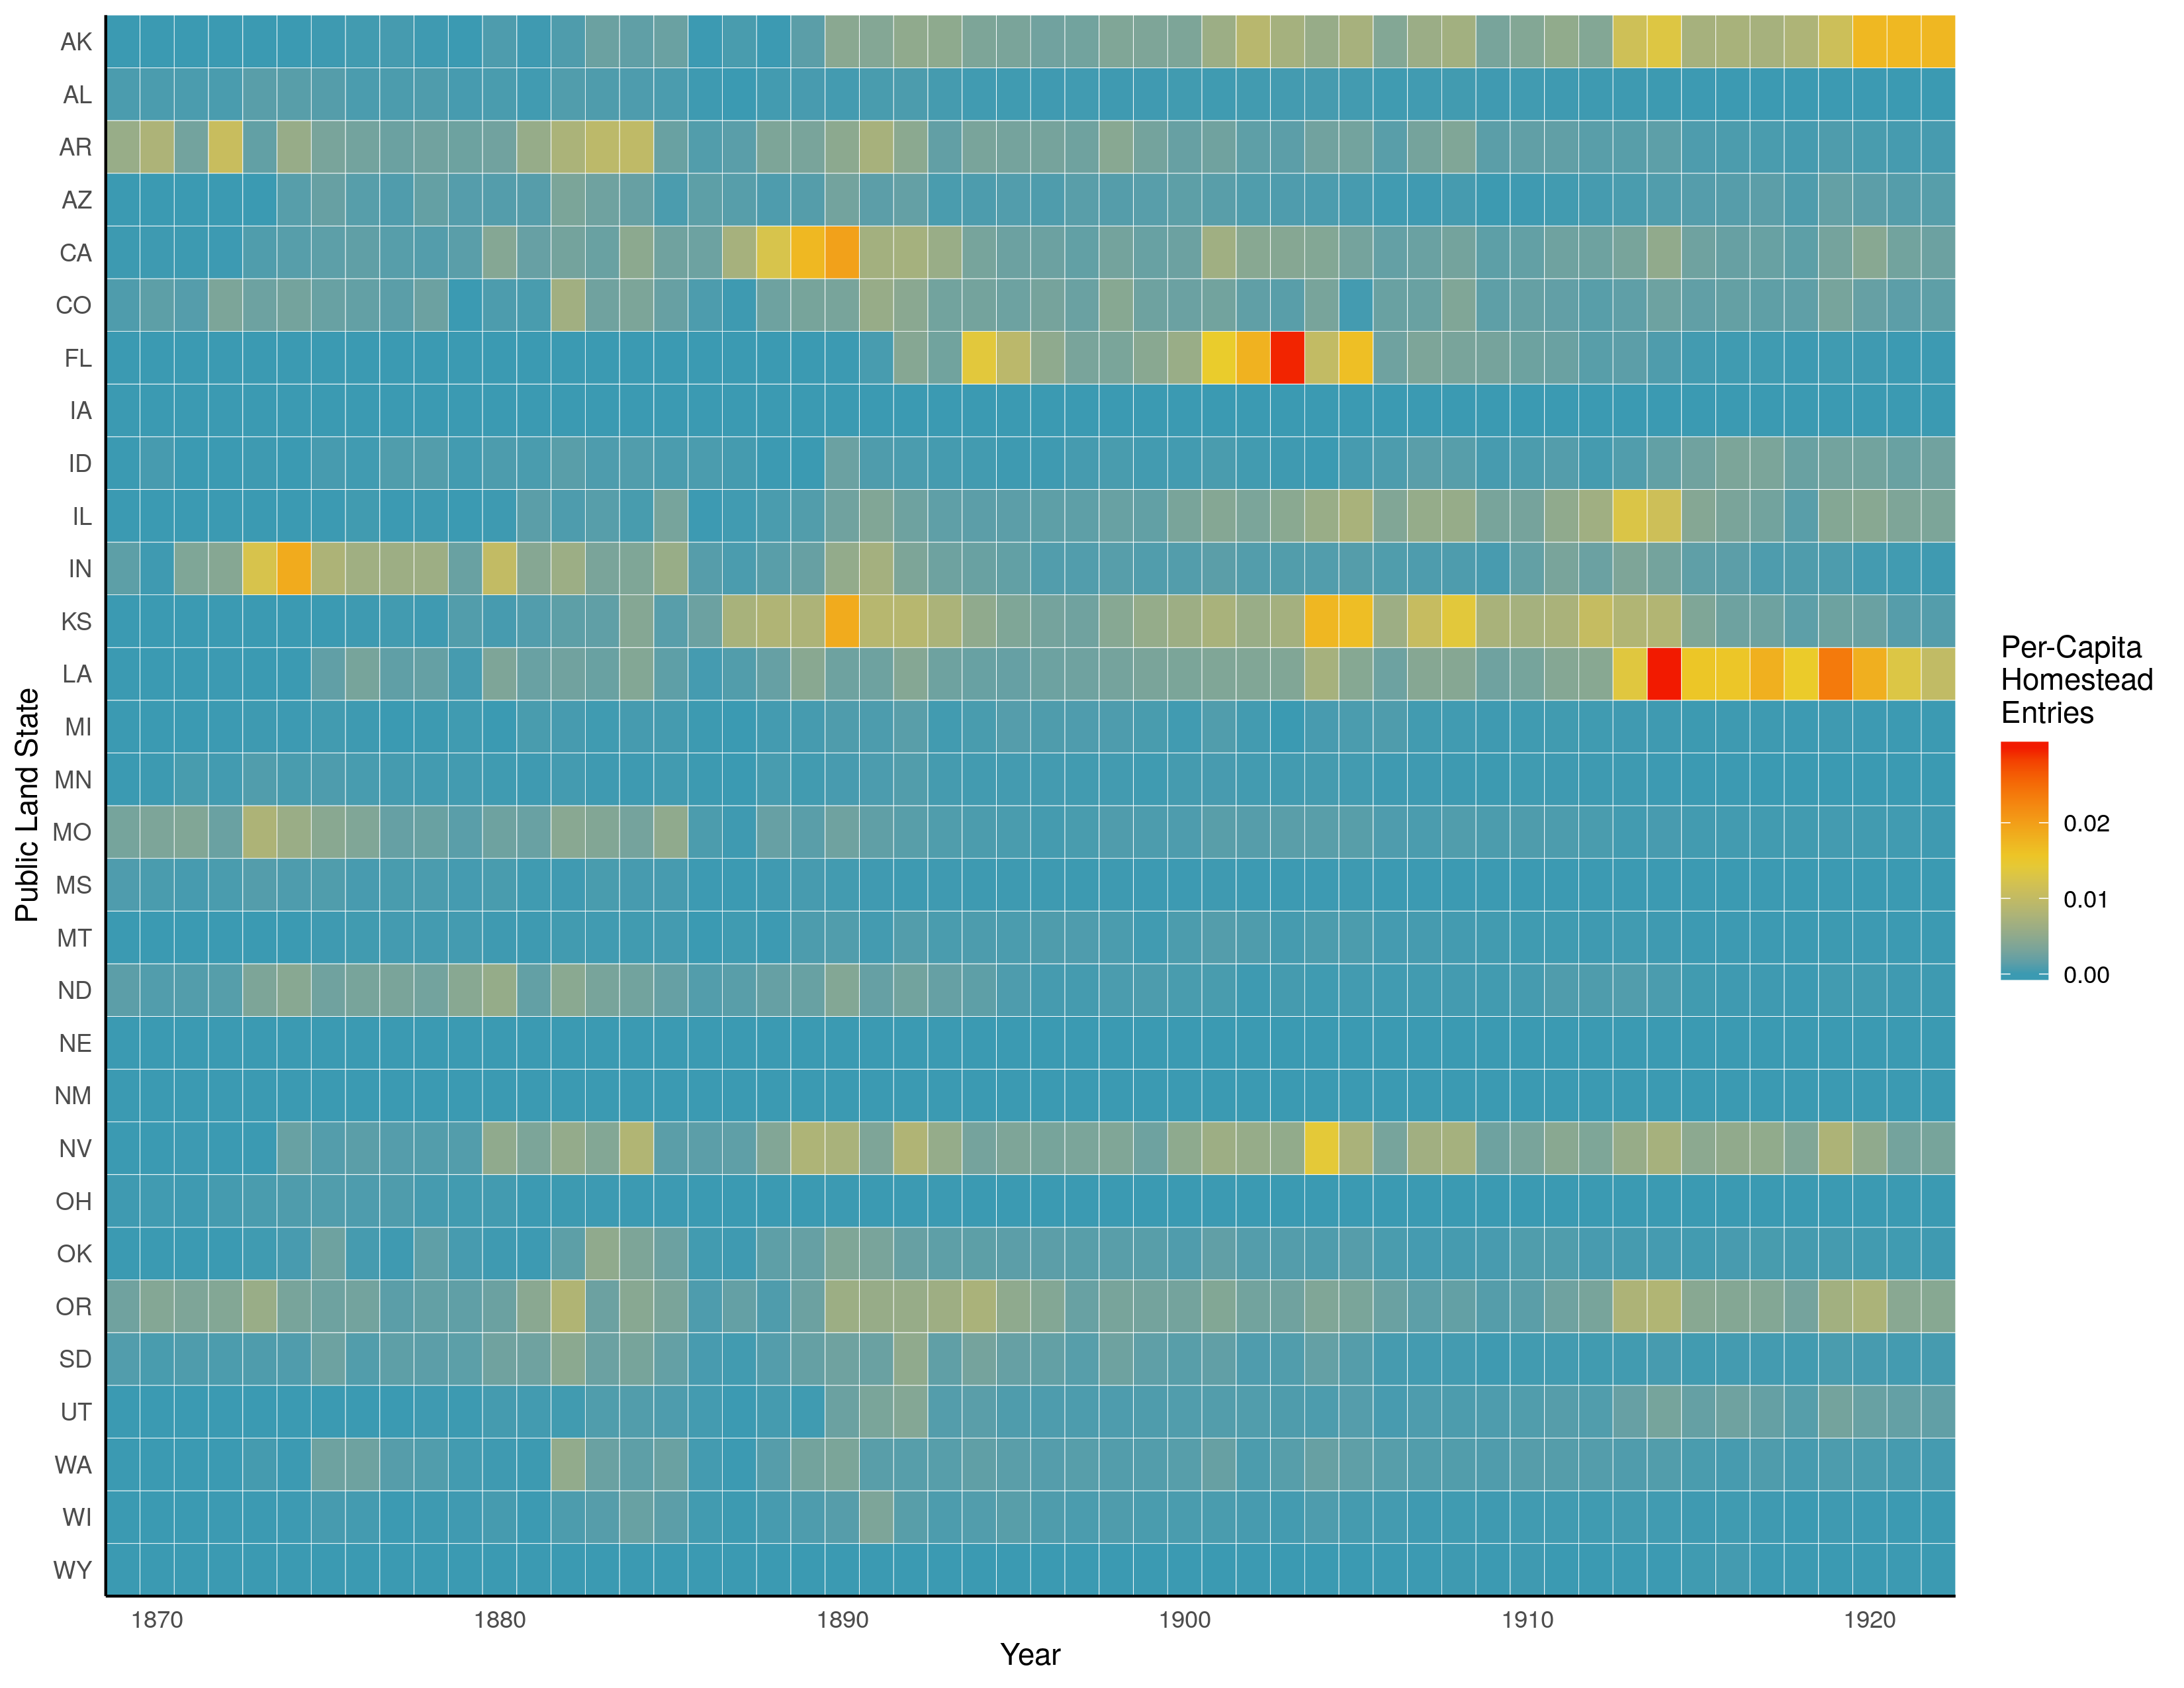
\includegraphics[width=\textwidth]{plots/homestead-heatmap.png}
	\end{center}
	\caption{Per-capita statewide sum of homestead entries in state $i$ and year $t$, 1869-1922. \label{fig:homestead-heatmap}}
\end{figure}

\begin{figure}[htbp]
	\begin{center}
		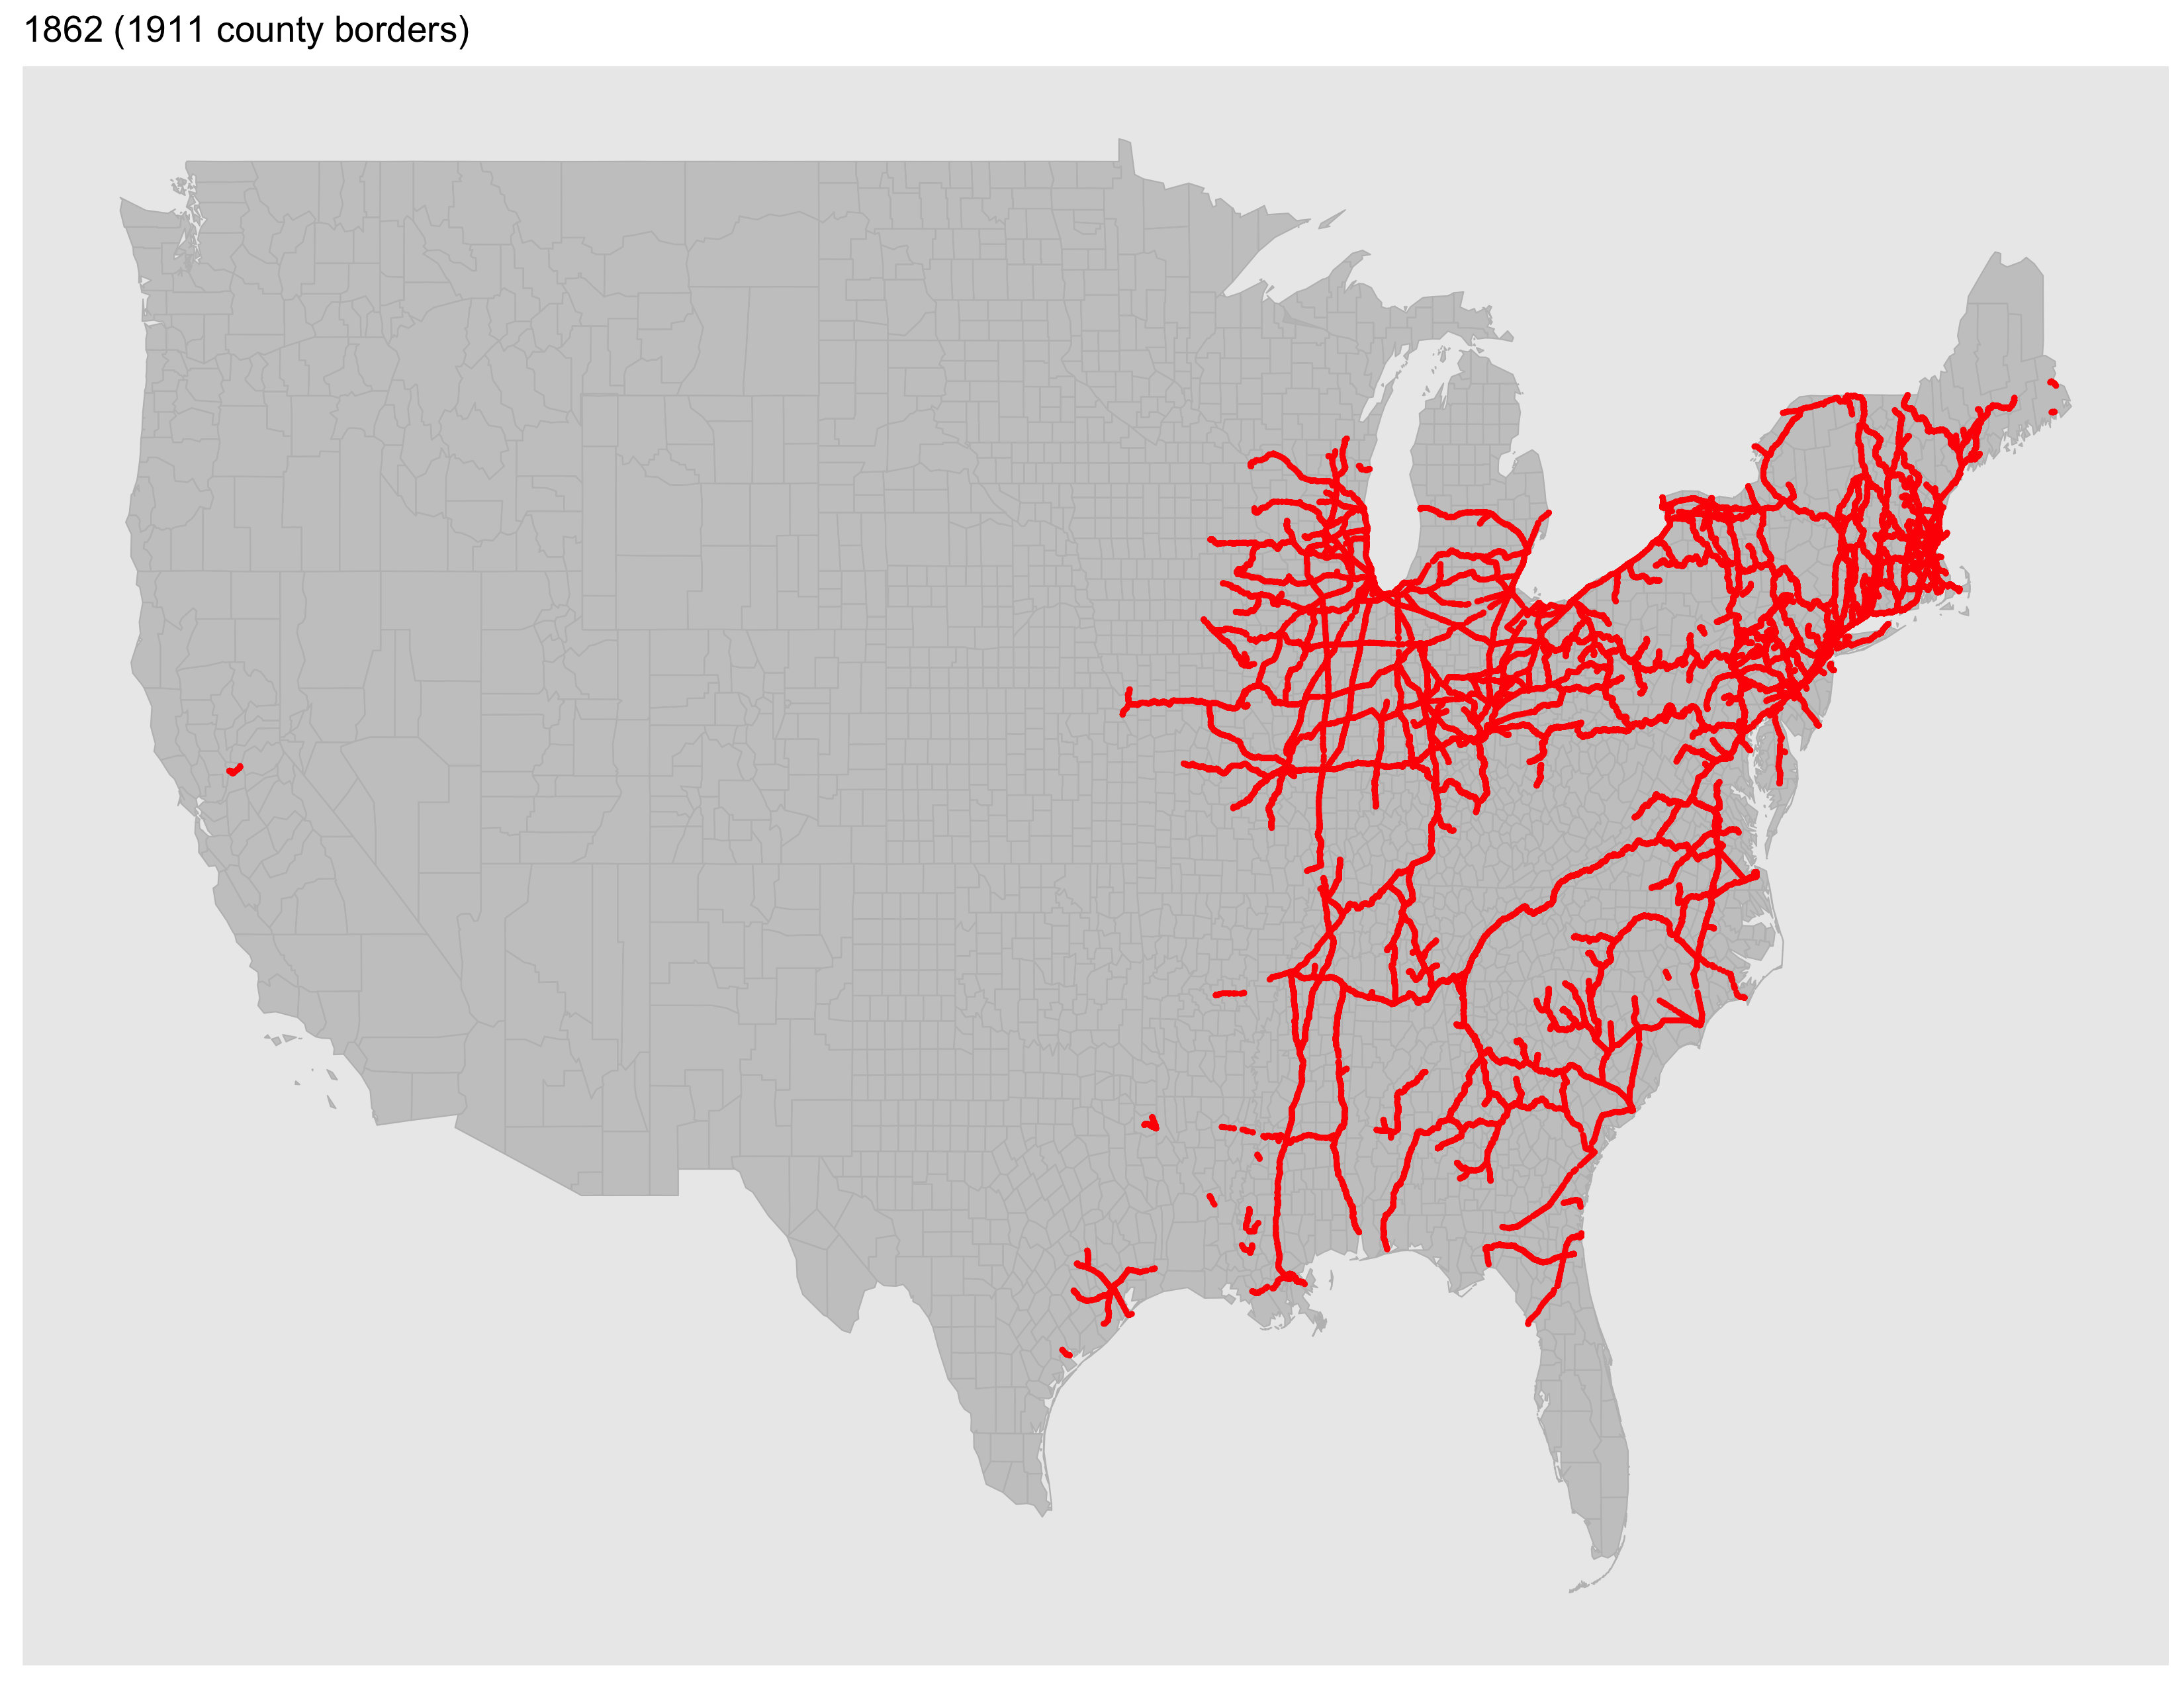
\includegraphics[width=0.7\textwidth]{plots/rr-1862.png} \\
		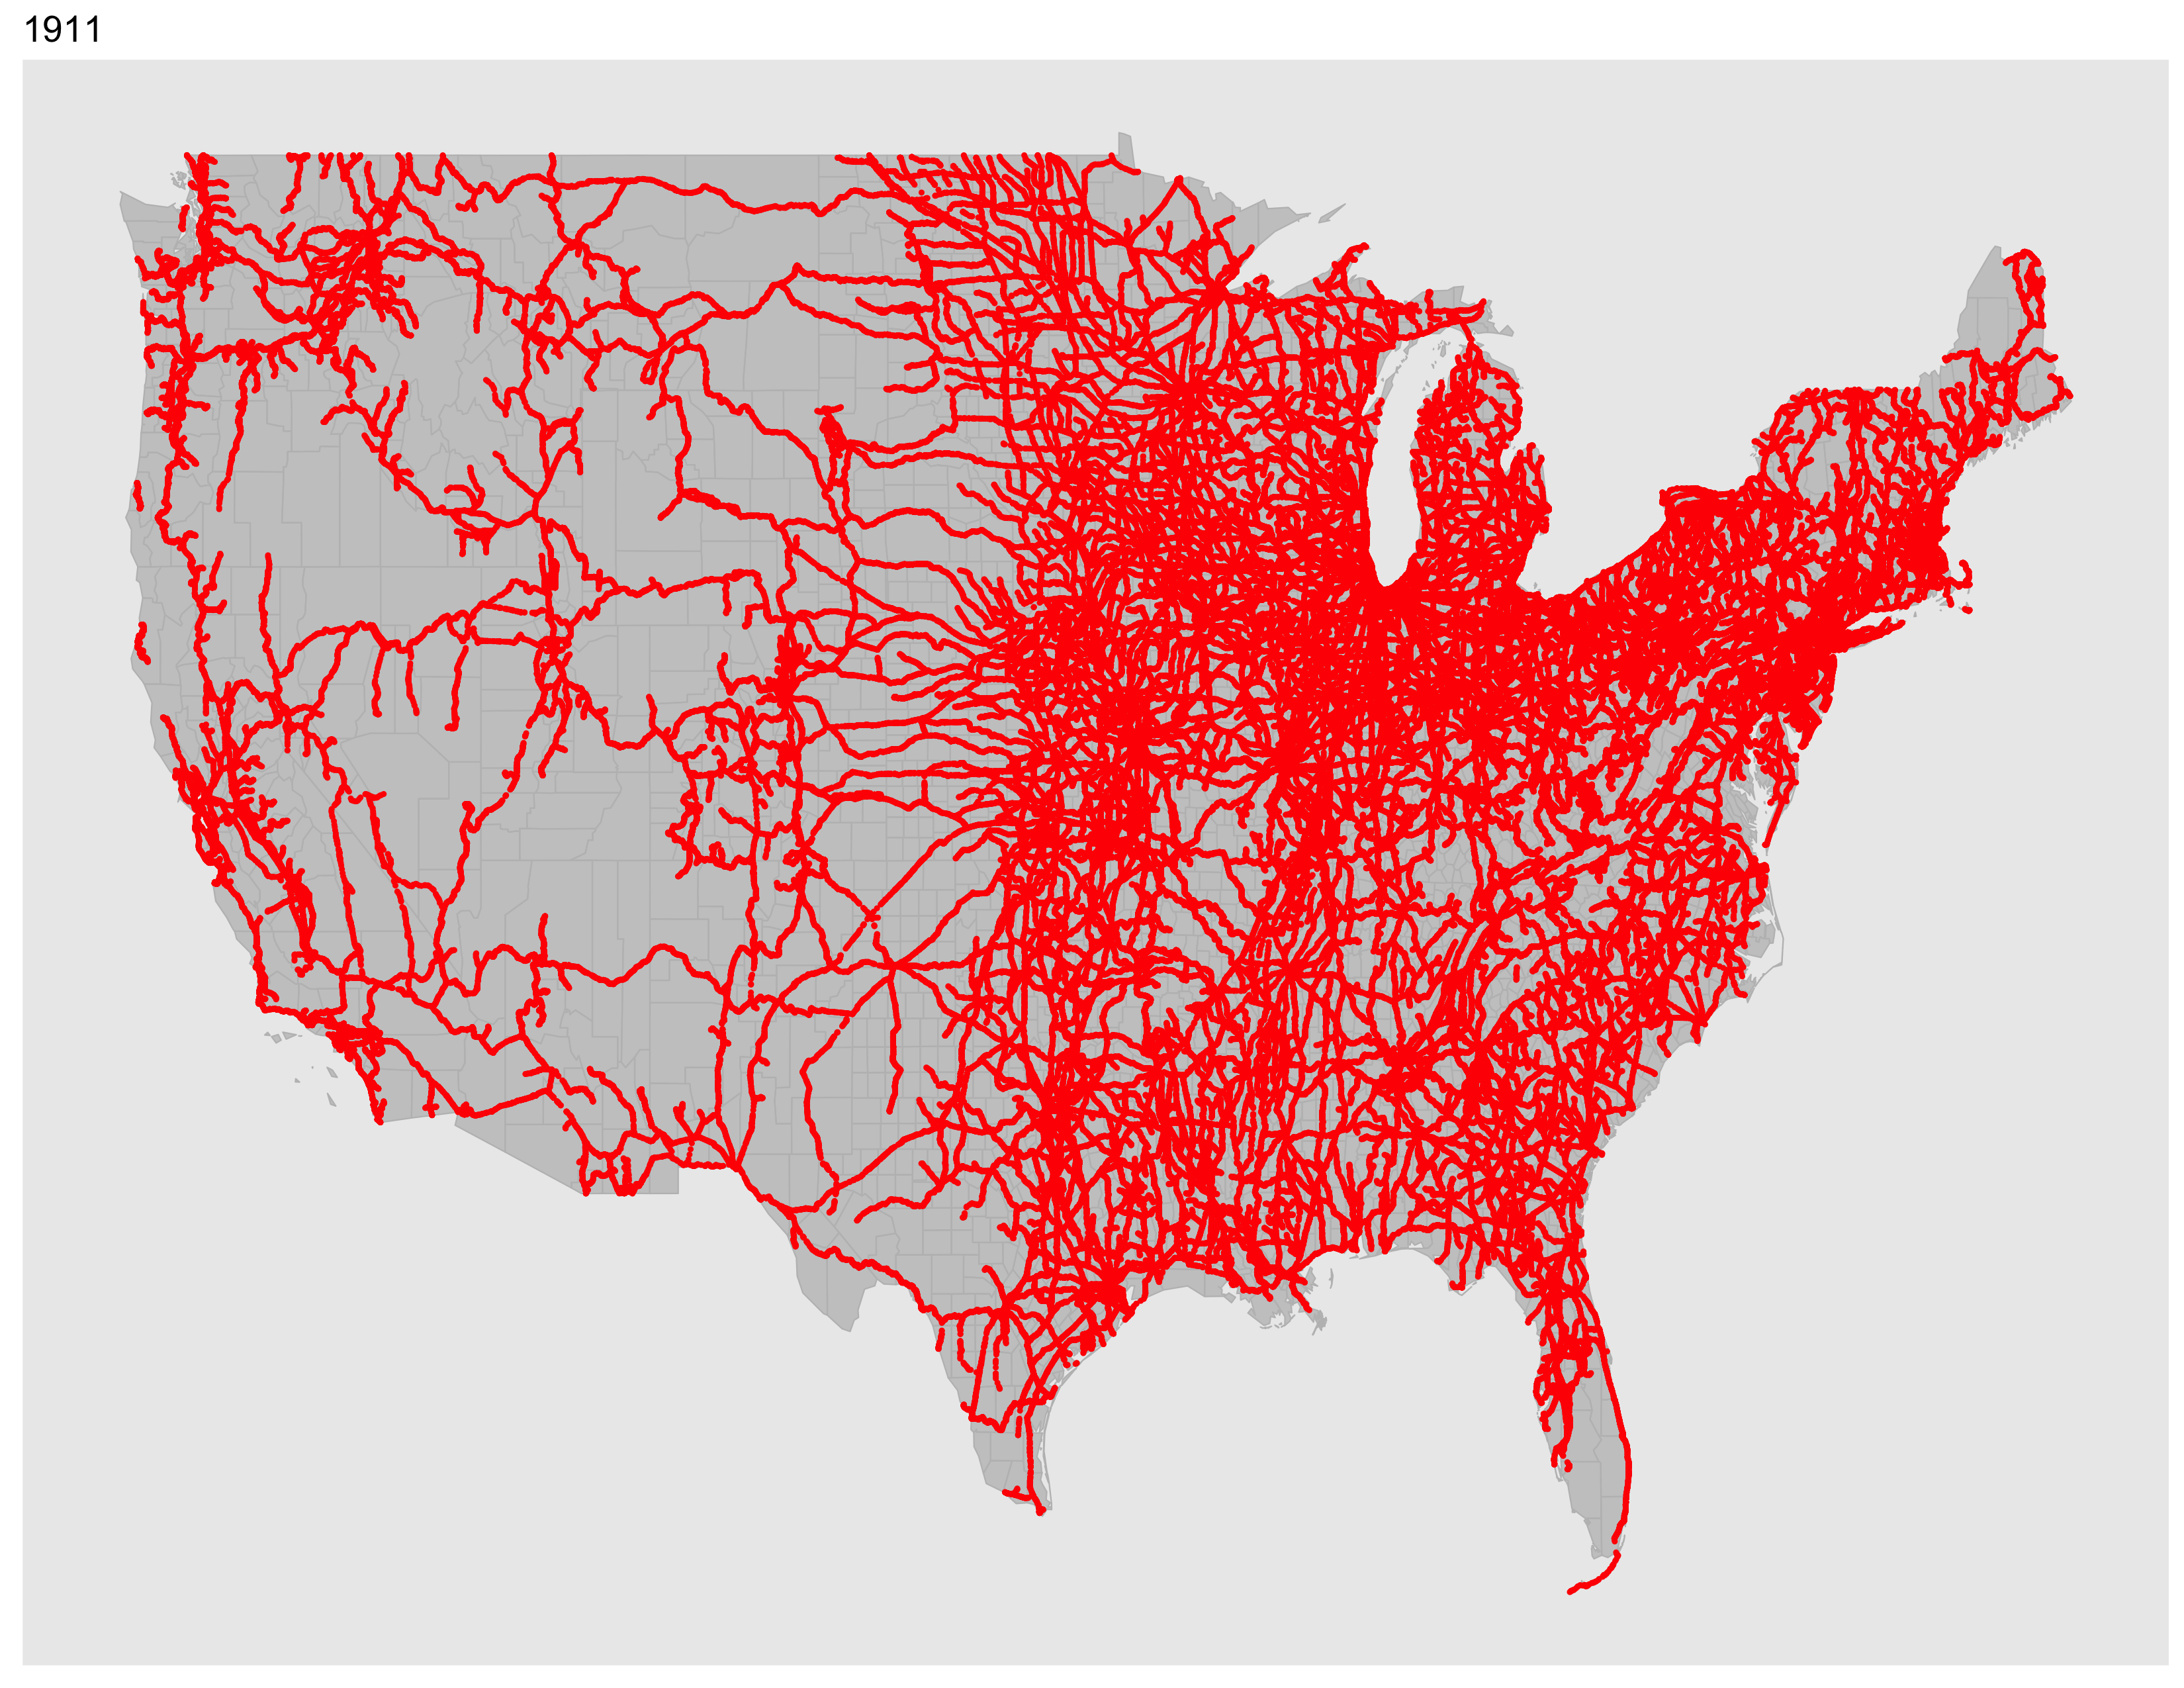
\includegraphics[width=0.7\textwidth]{plots/rr-1911.png} \\
	\end{center}
	\caption{Railroad lines in 1862 and 1911, overlaid on 1911 county borders. Railroad data from \cite{atack2013use} and county border data from \cite{long1995atlas}. \label{rr-map}} 
\end{figure}

\pagebreak
\section{Simulations} \label{sims-sm}

\begin{figure}[htbp]
	\centering
	\begin{subfigure}[t]{0.48\textwidth}
		\centering
		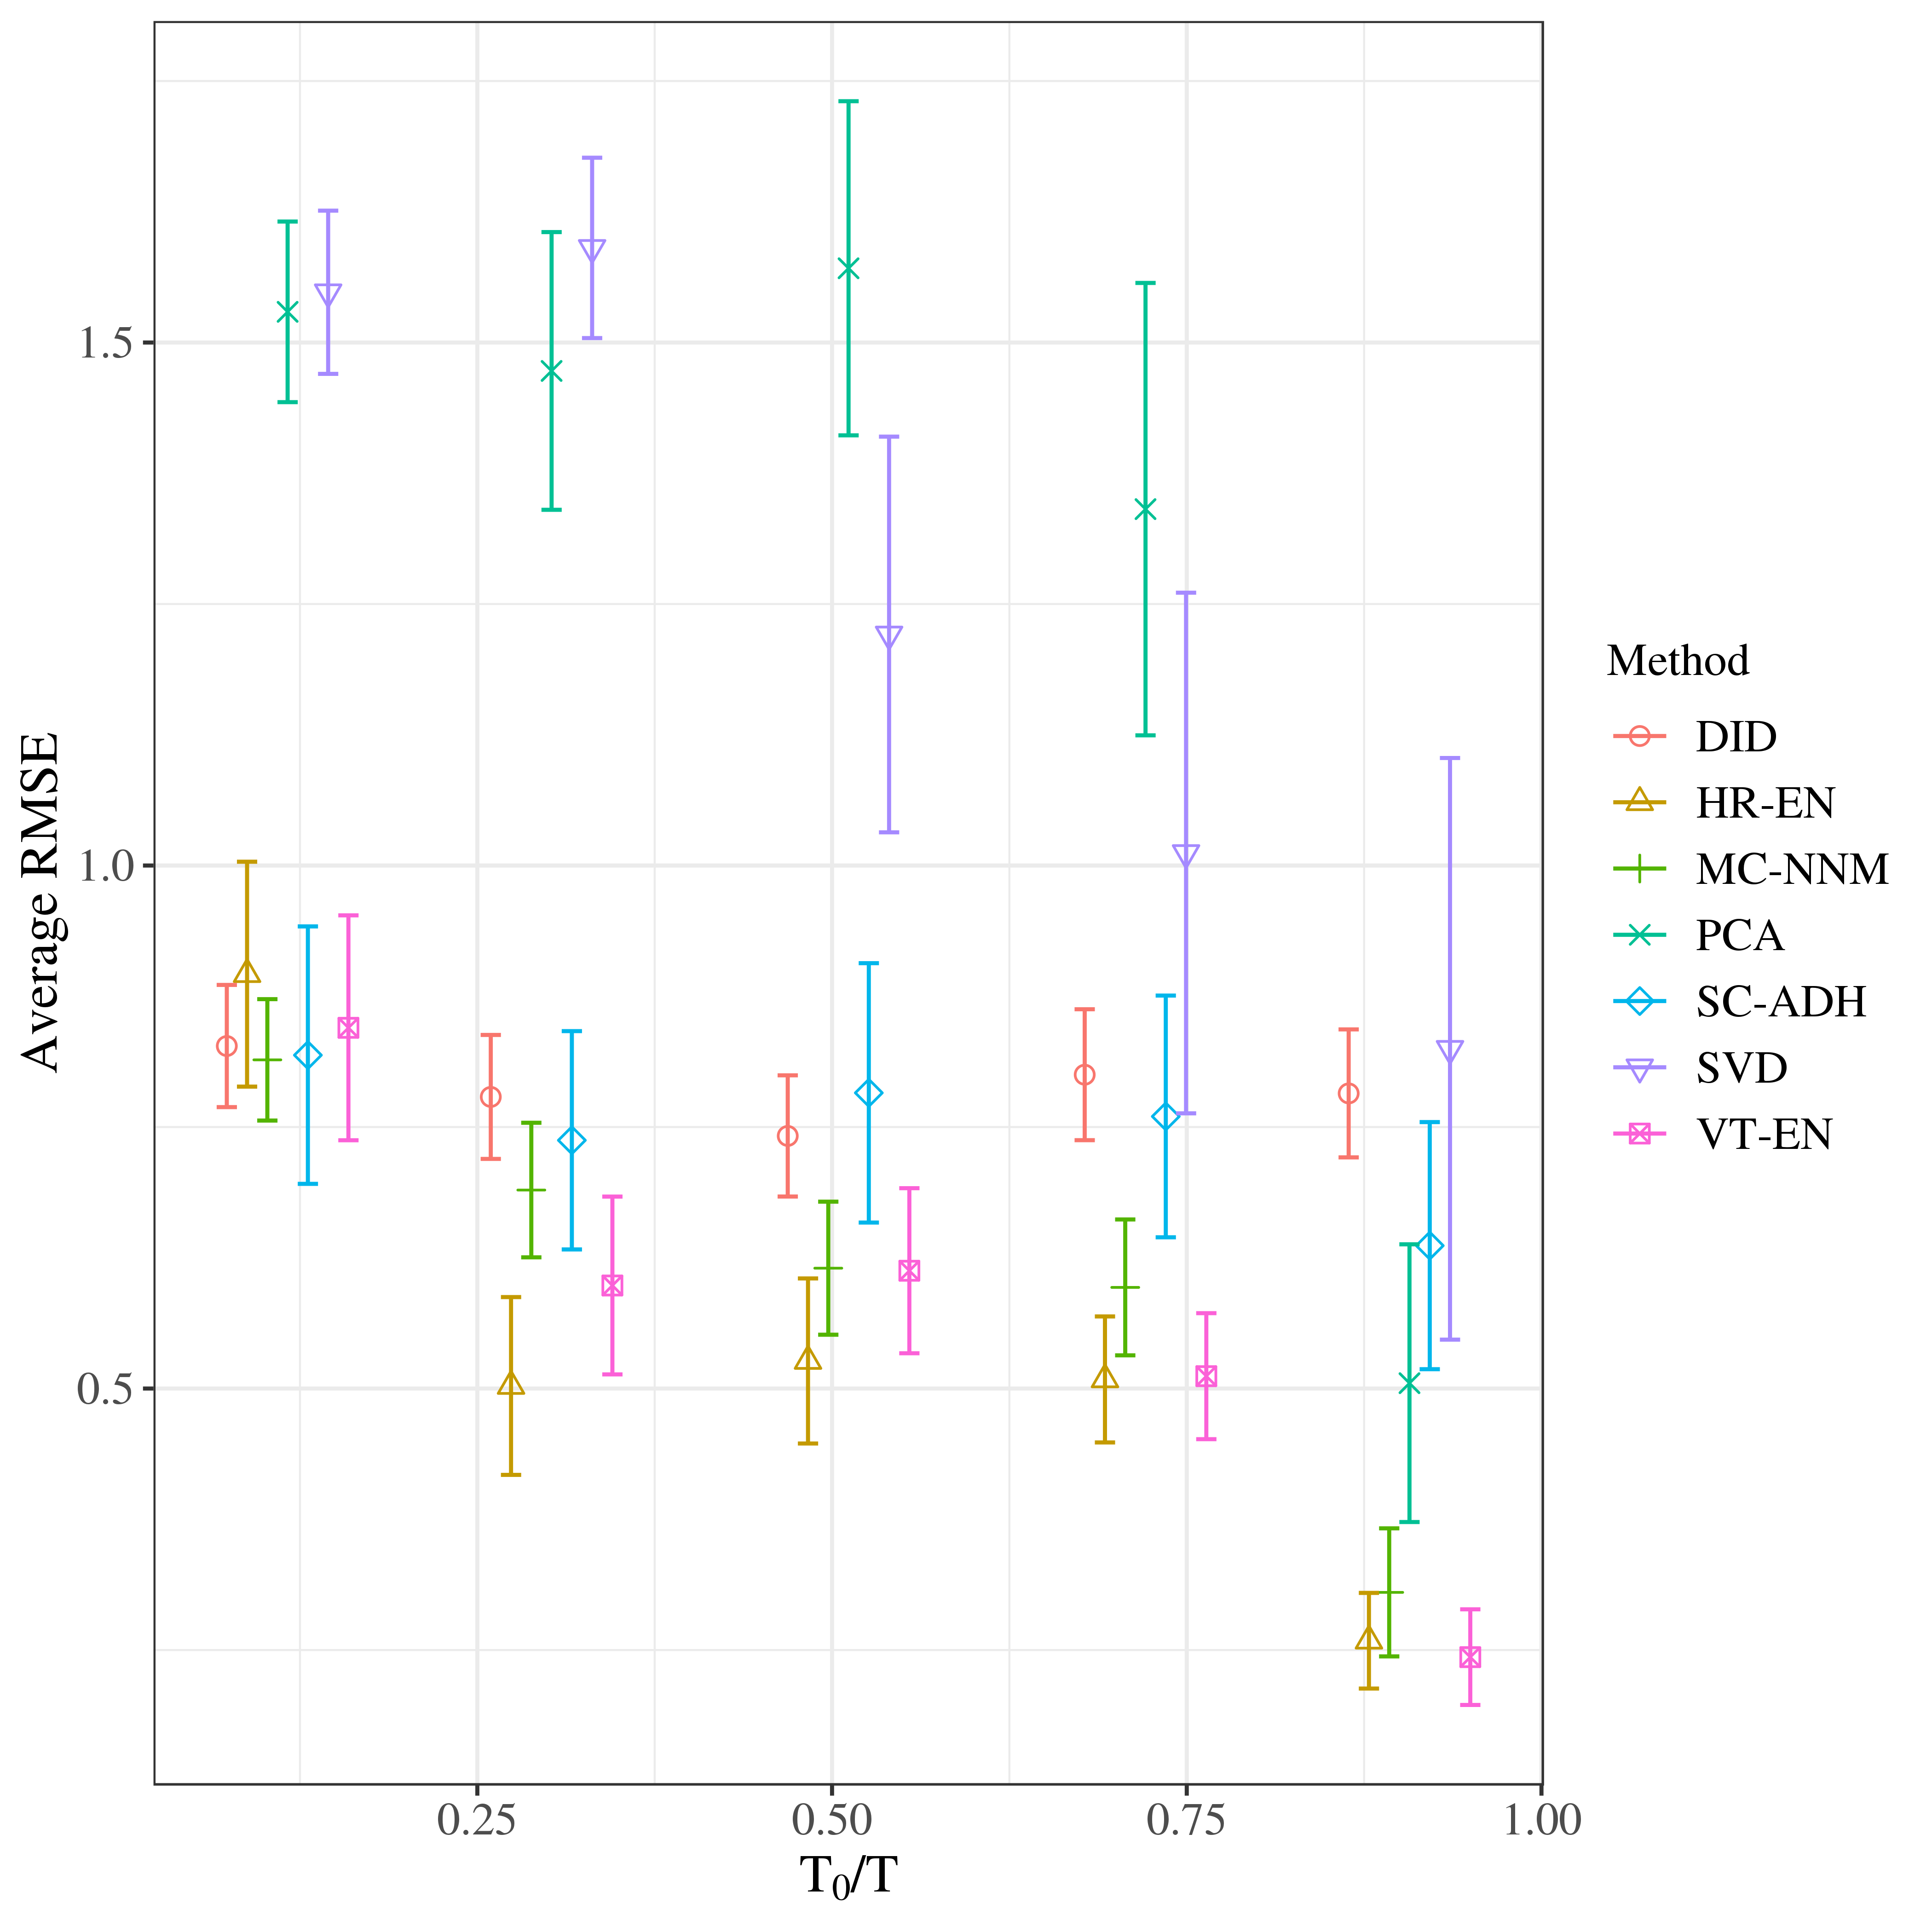
\includegraphics[width=\textwidth]{plots/basque_N_16_T_43_numruns_20_num_treated_8_simultaneuous_1.png}
		\caption{Basque Country terrorism data, $N_t = 8$} 
	\end{subfigure}
	~ 
	\begin{subfigure}[t]{0.48\textwidth}
		\centering
		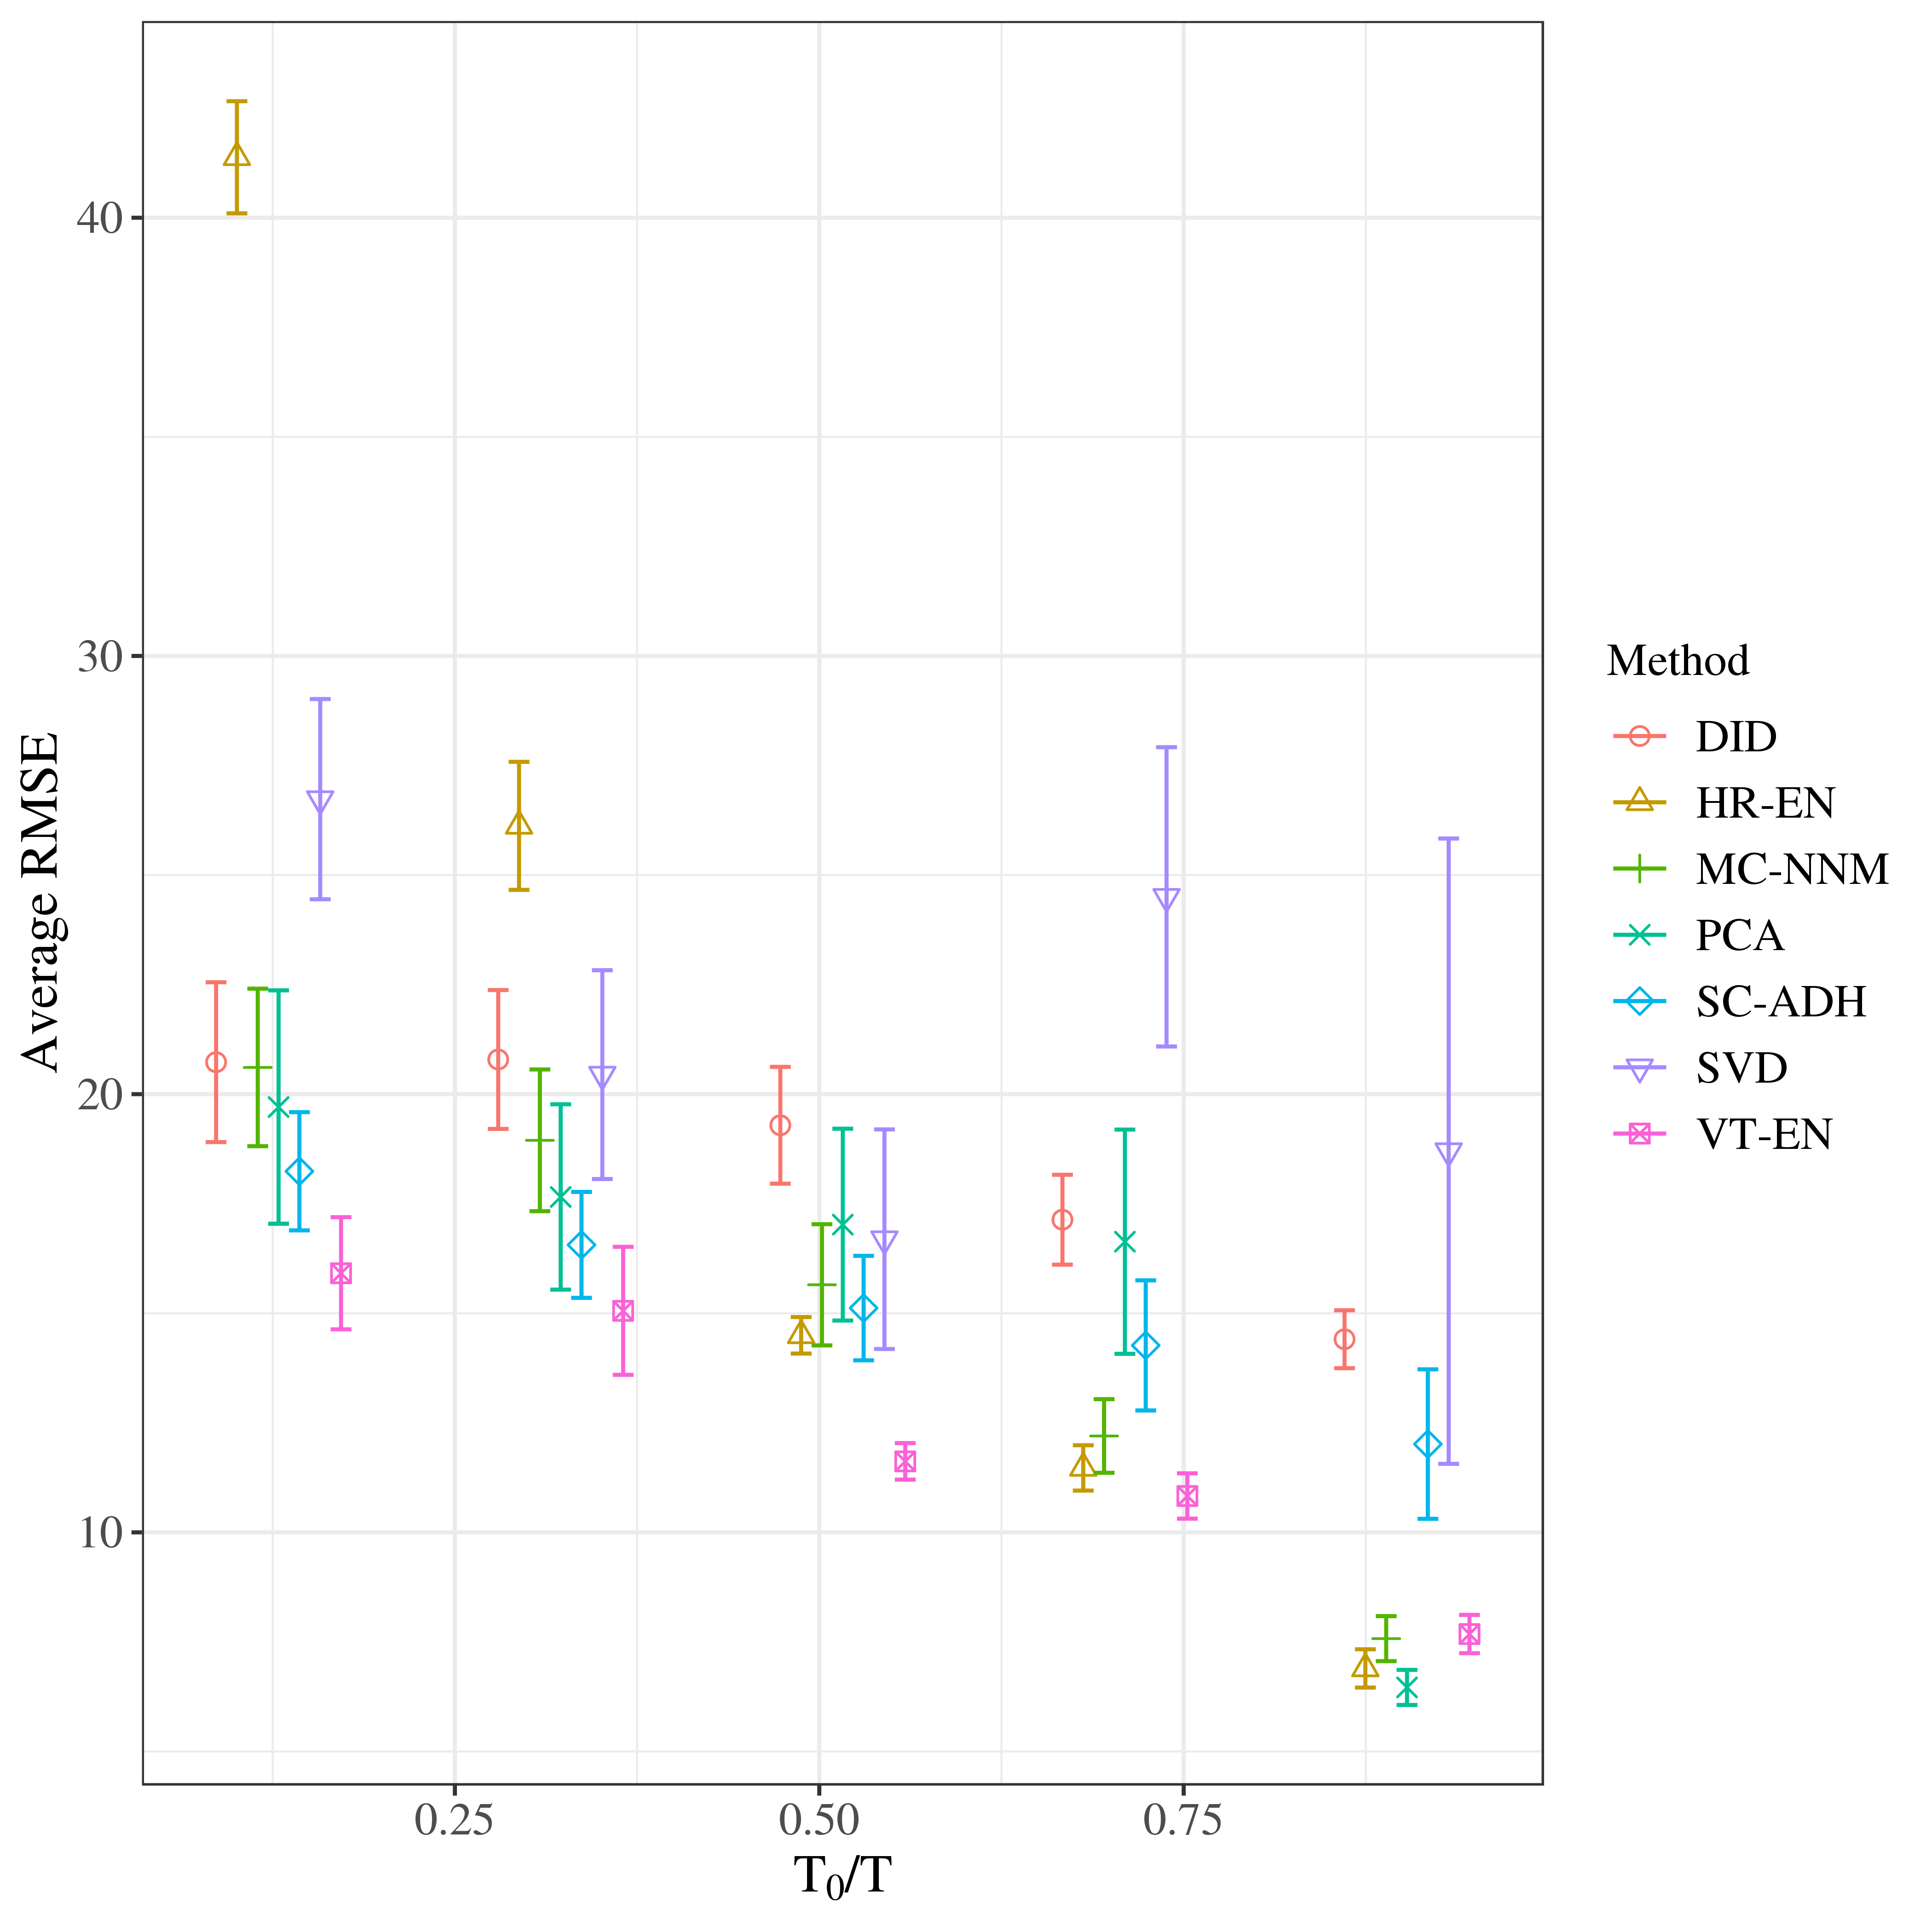
\includegraphics[width=\textwidth]{plots/california_N_38_T_31_numruns_20_num_treated_19_simultaneuous_1.png}
		\caption{California smoking ban data, $N_t = 19$}
	\end{subfigure}
	~
	\begin{subfigure}[t]{0.48\textwidth}
		\centering
		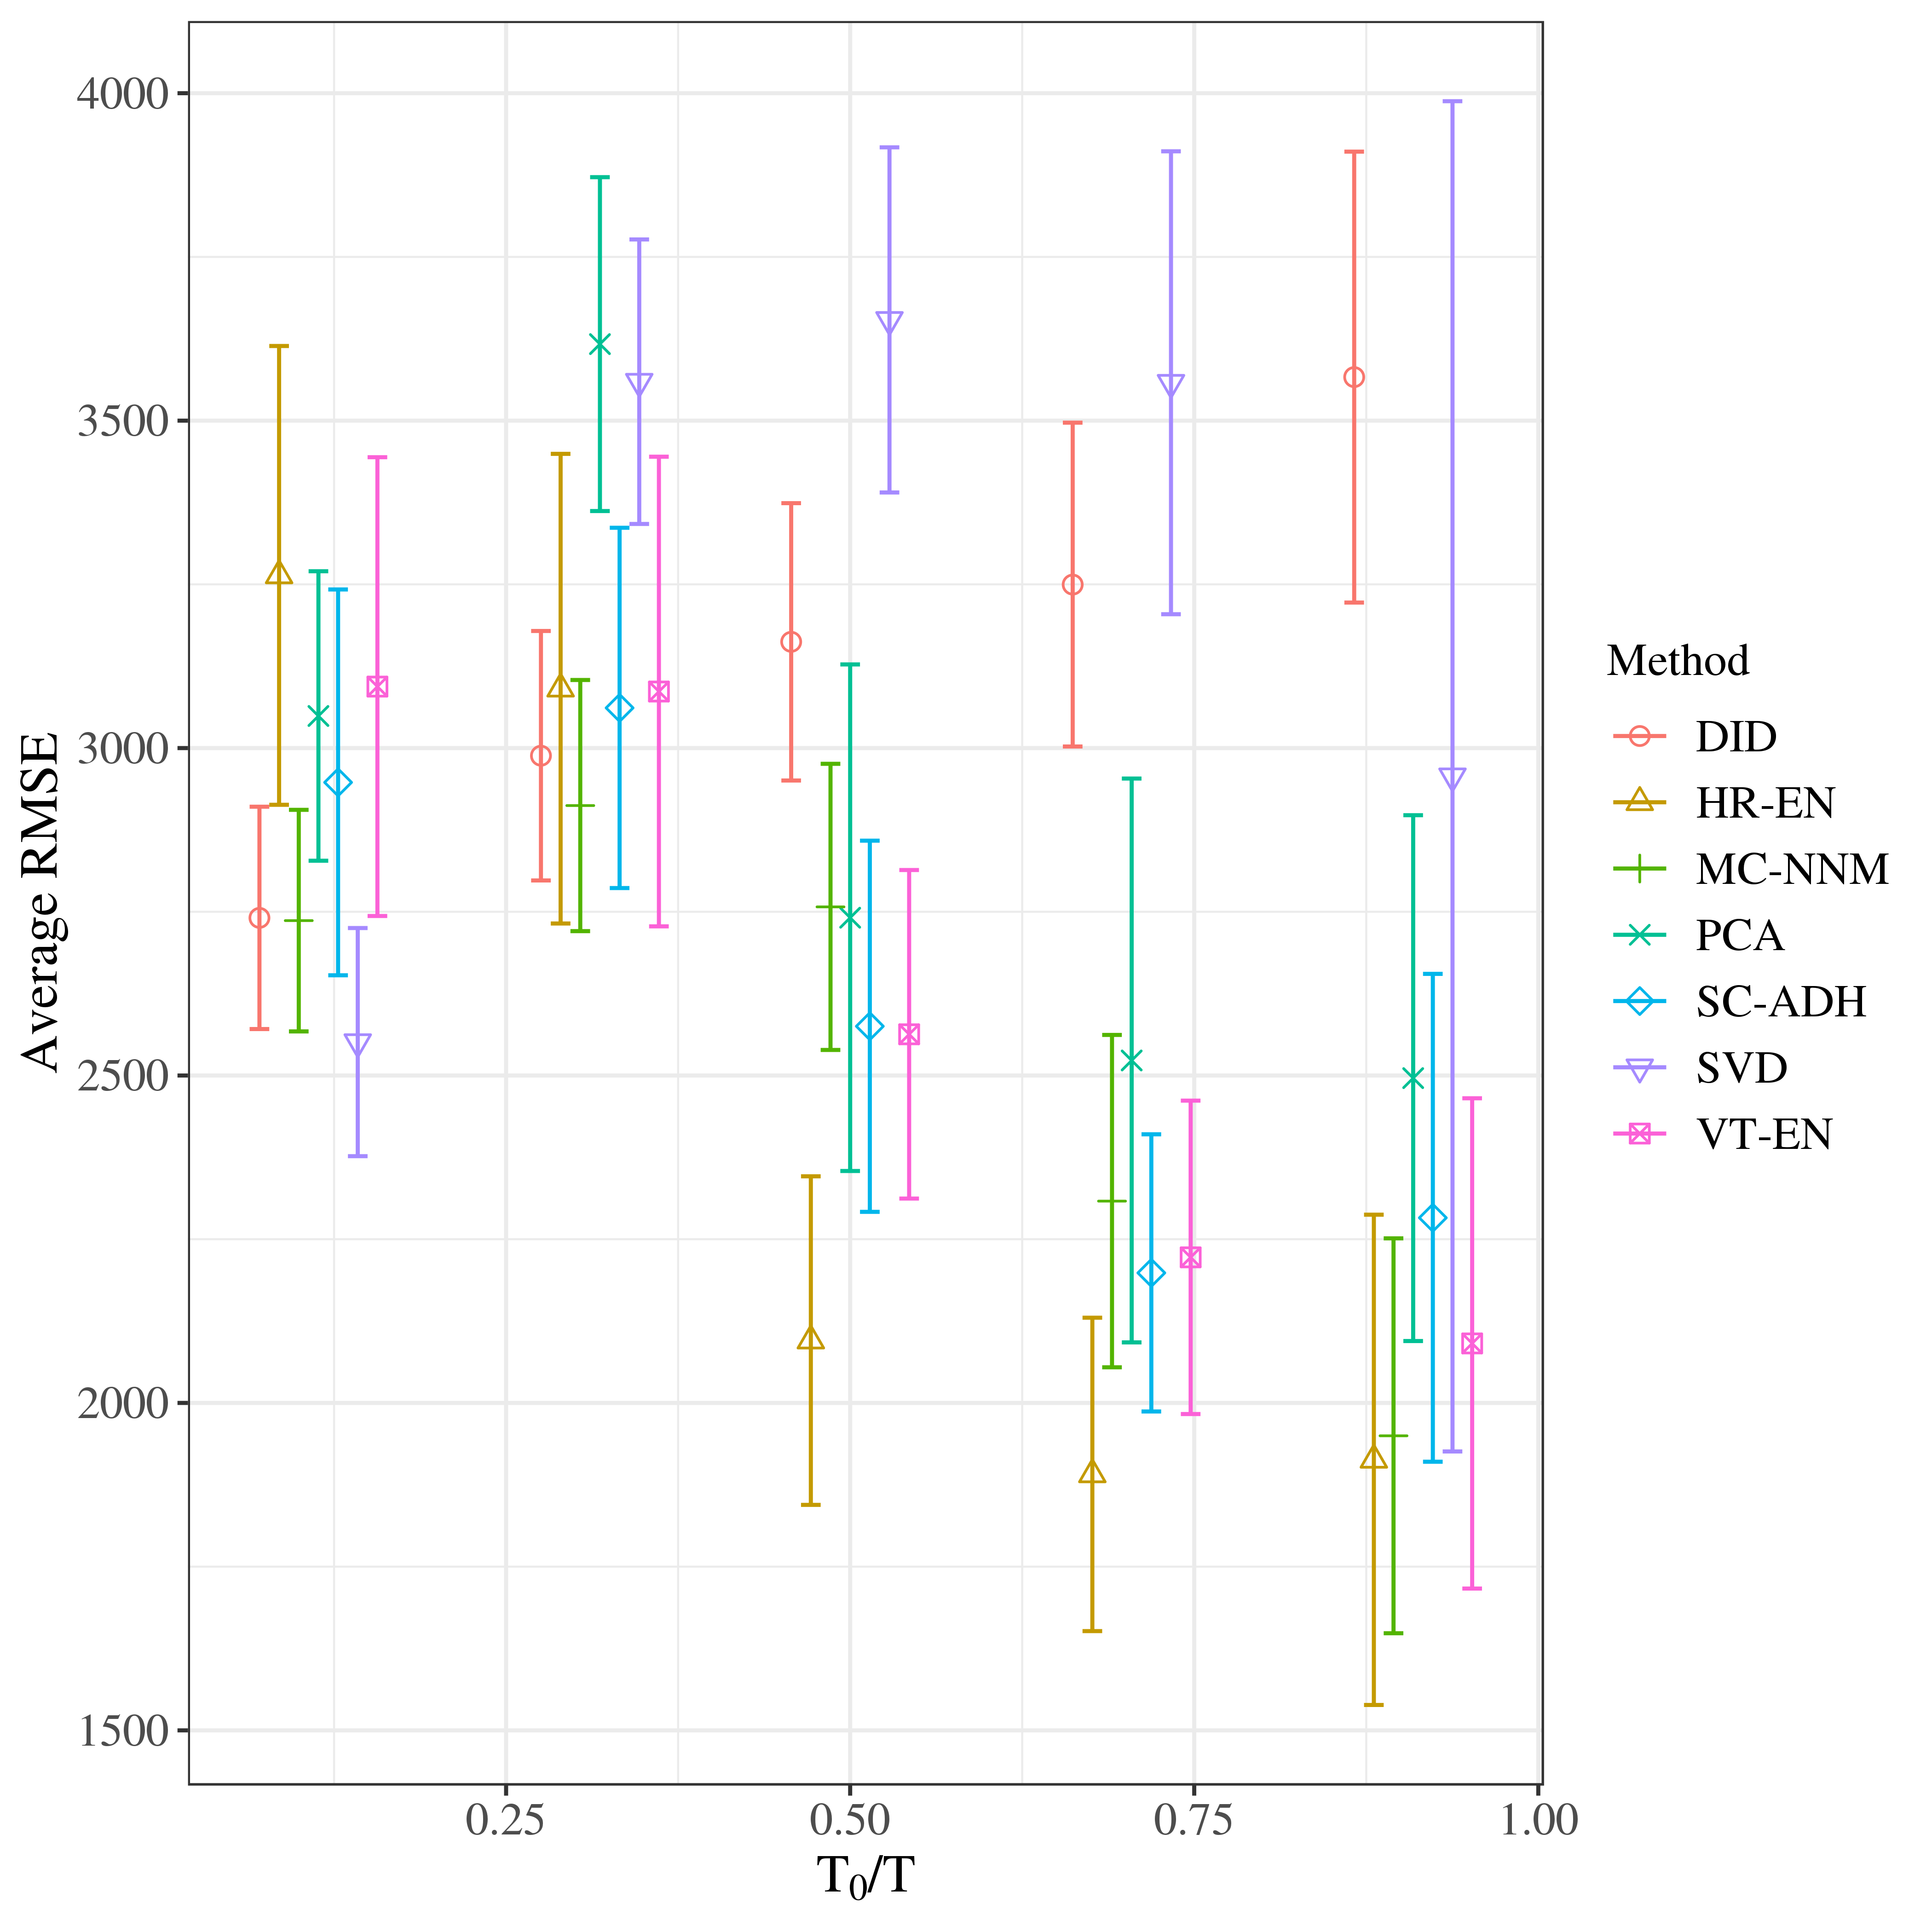
\includegraphics[width=\textwidth]{plots/germany_N_16_T_44_numruns_20_num_treated_8_simultaneuous_1.png}
		\caption{West German reunification data, $N_t = 8$} 
	\end{subfigure}
	\caption{Placebo tests under simultaneous treatment adoption. See footnotes to Fig. \ref{synth-stag}. \label{synth-sim}} 
\end{figure}

\begin{figure}[htbp]
	\centering
%	\begin{subfigure}[t]{0.48\textwidth}
%		\centering
%		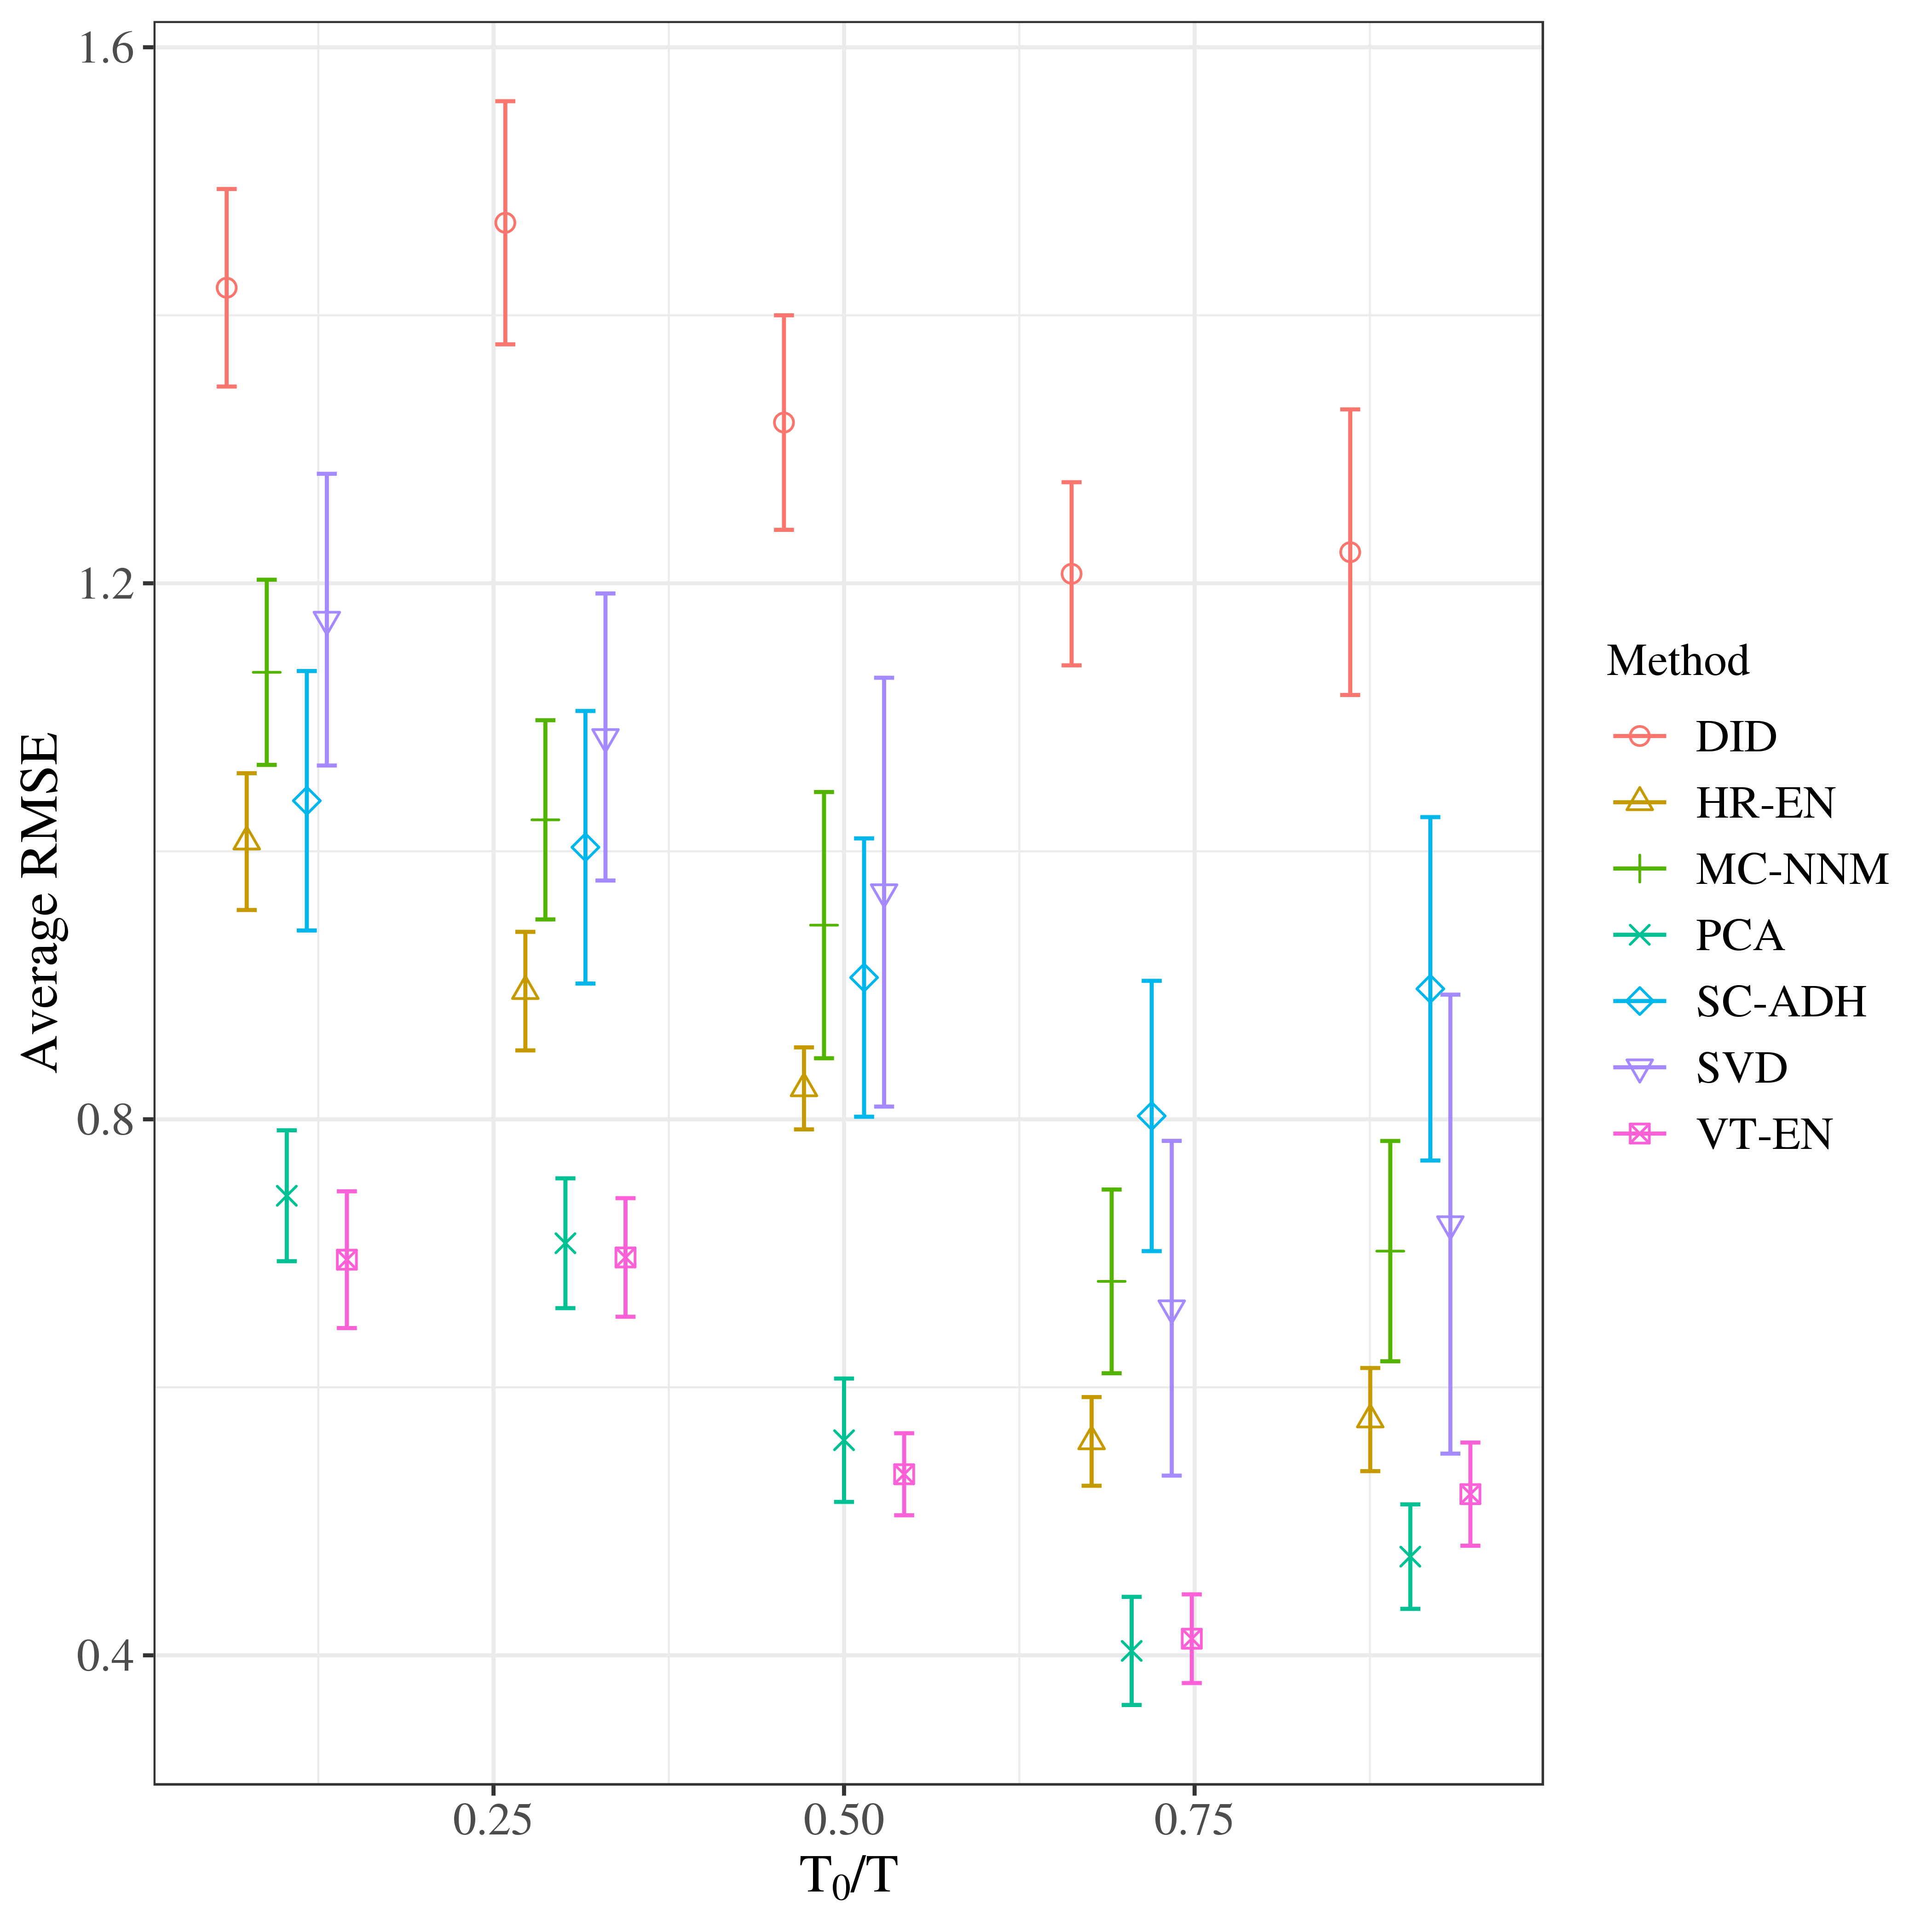
\includegraphics[width=\textwidth]{plots/educ_pc_N_19_T_156_numruns_20_num_treated_10_simultaneuous_0.png}
%		\caption{State government education spending, $N_t = 10$}
%	\end{subfigure}
%	~ 
%		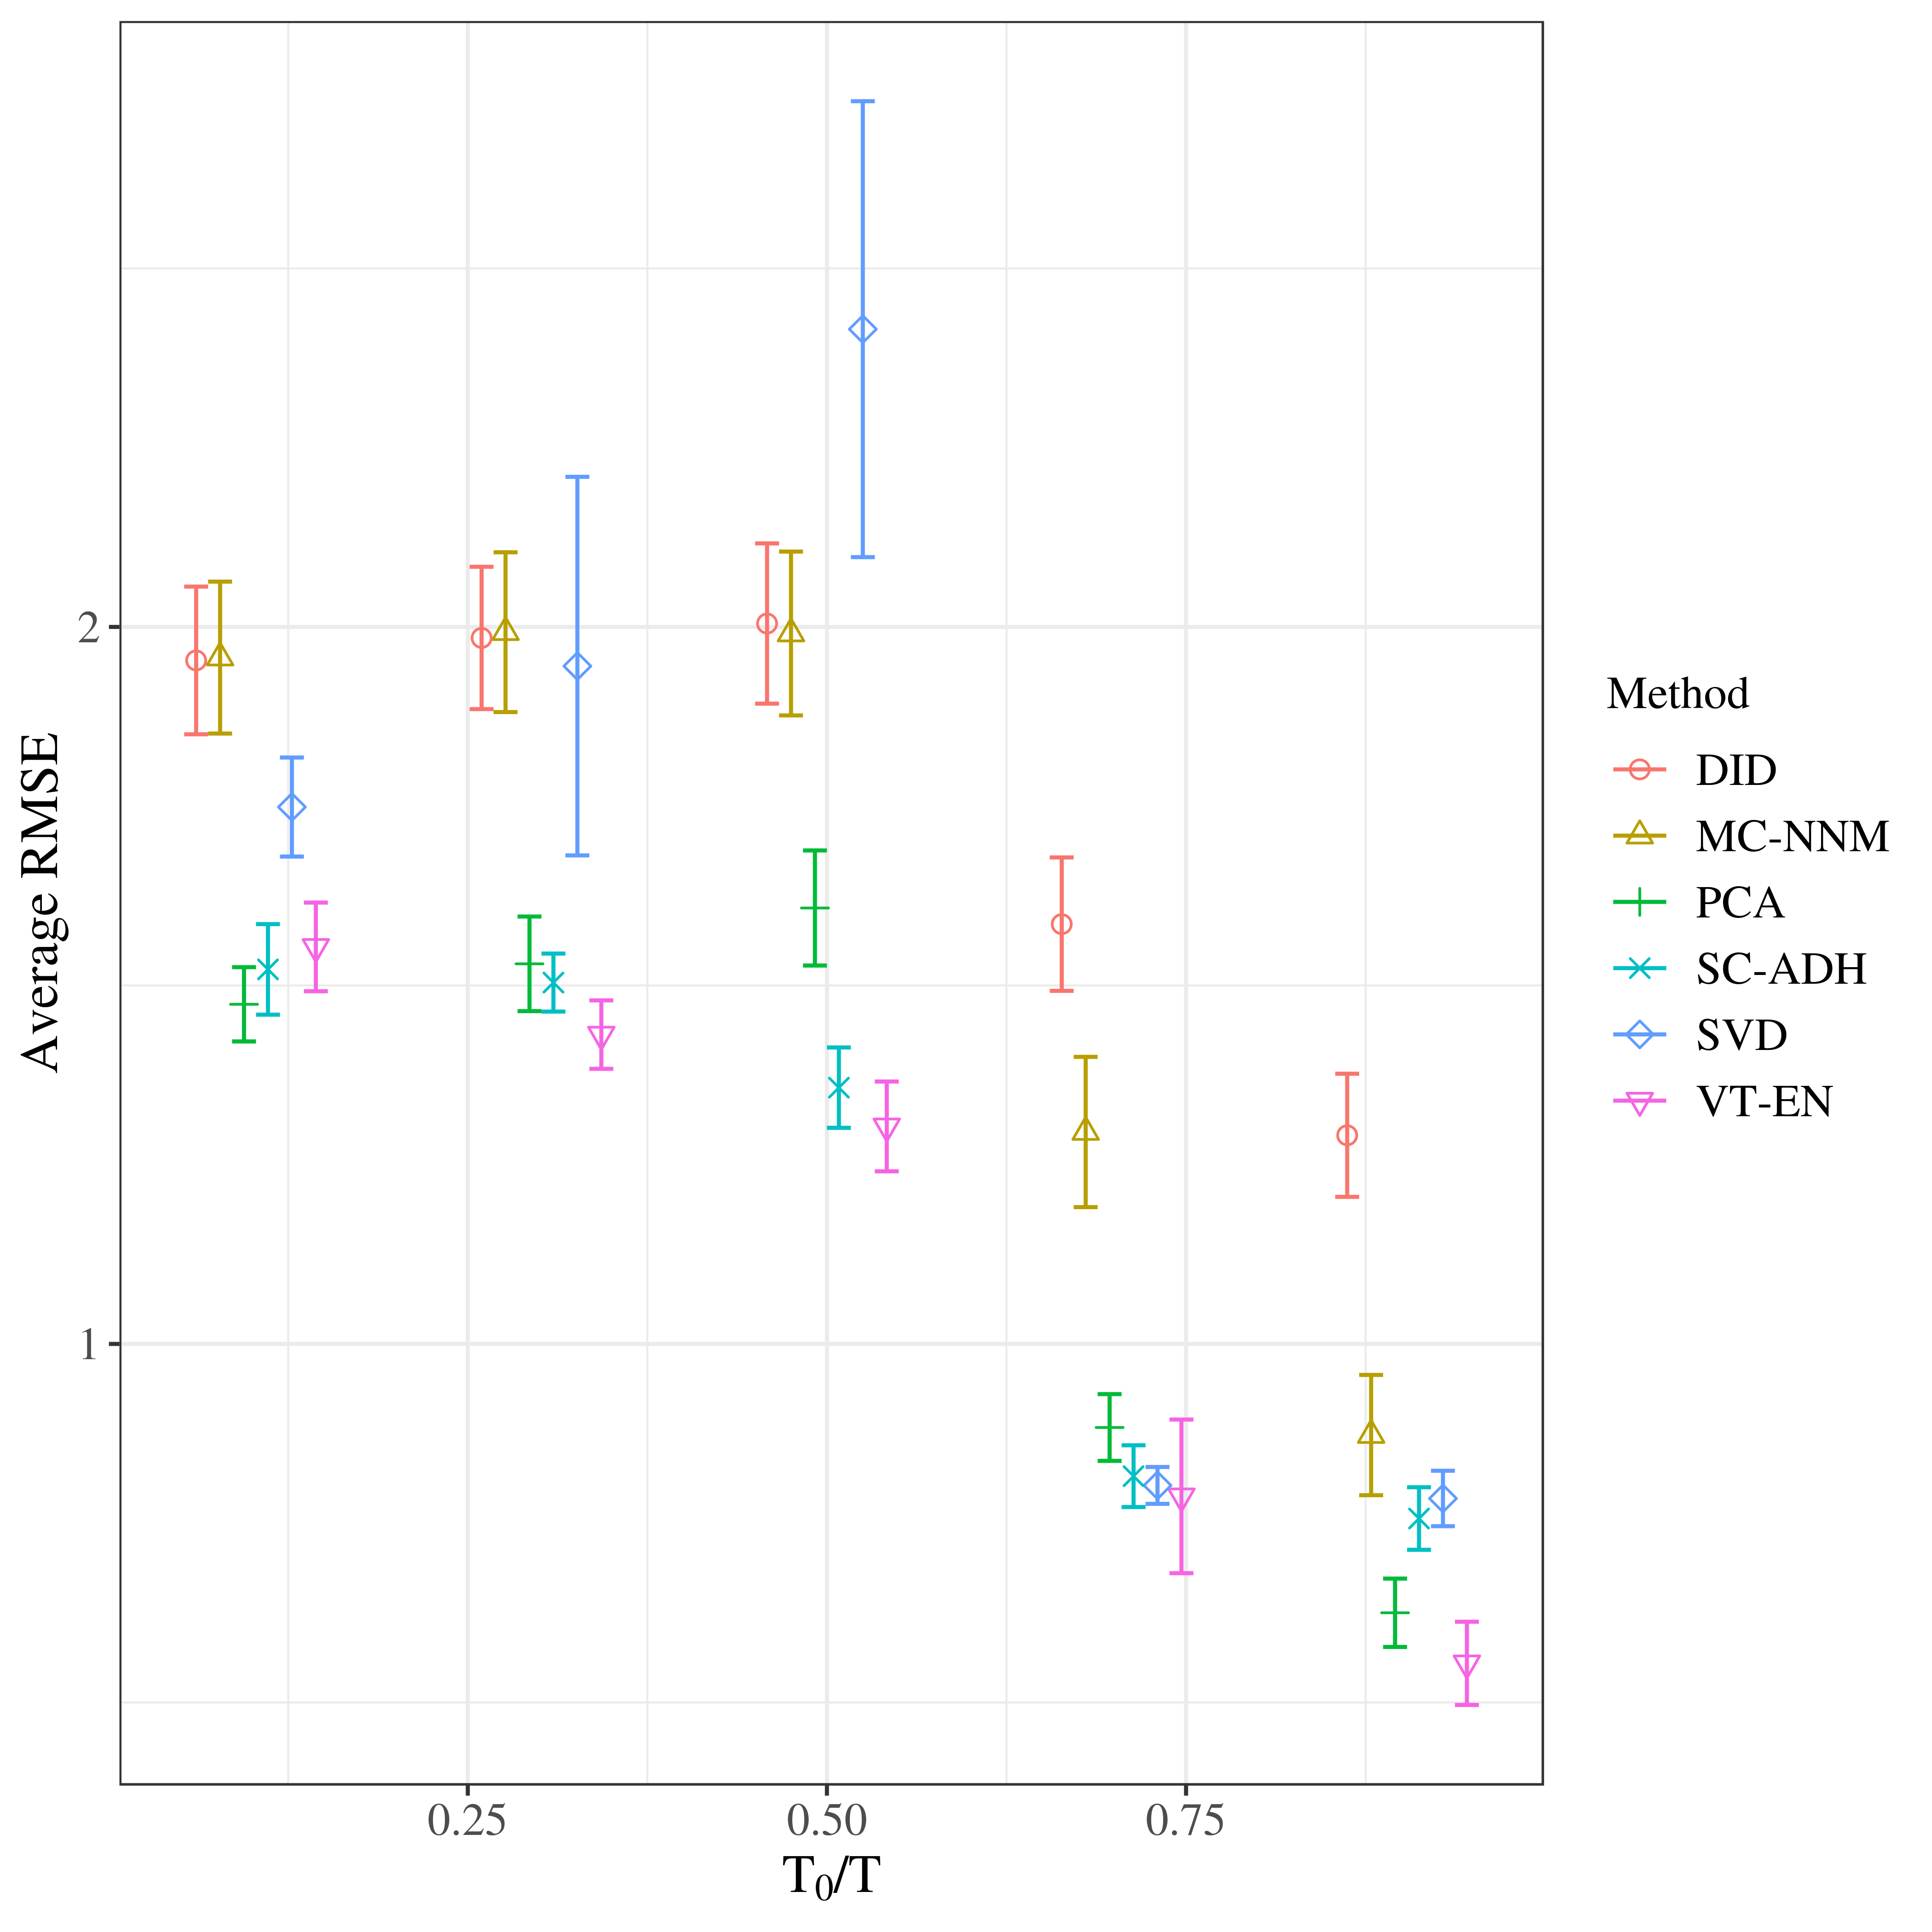
\includegraphics[width=\textwidth]{plots/educ_pc_N_17_T_156_numruns_20_num_treated_9_simultaneuous_1.png}
%		\caption{State government education spending, $N_t = 9$}
%	\end{subfigure}
	\begin{subfigure}[t]{0.48\textwidth}
		\centering
		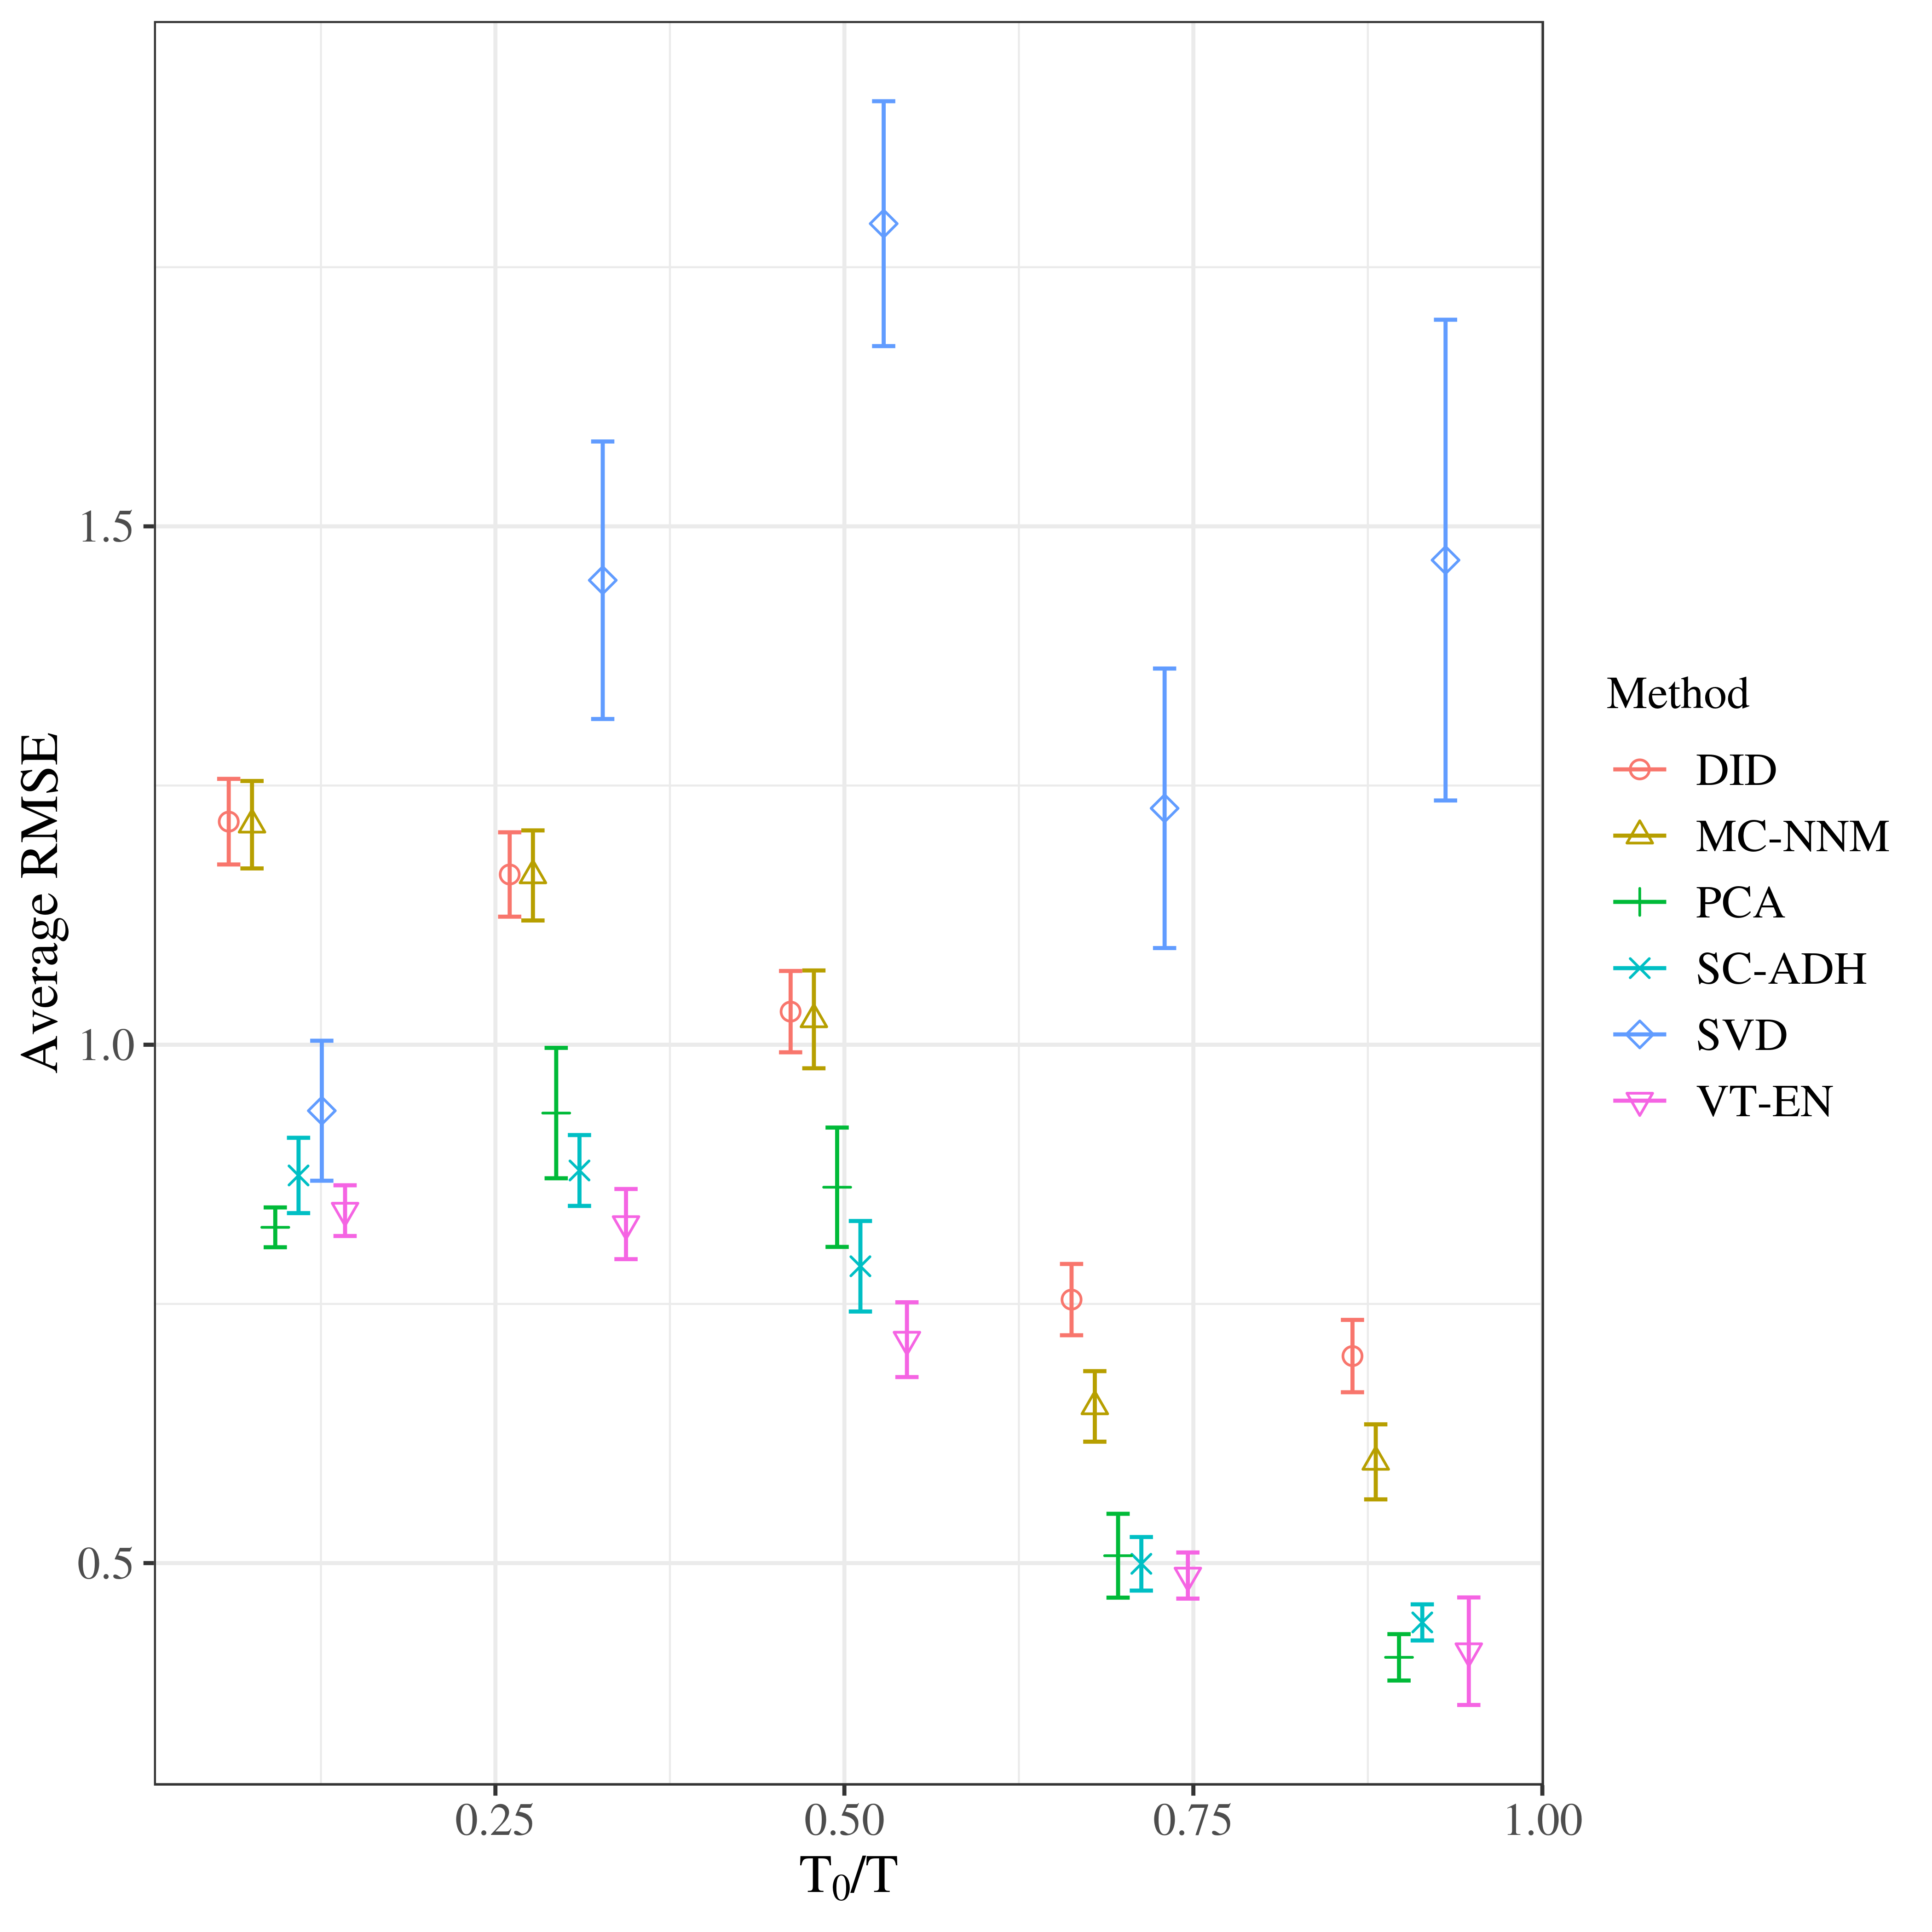
\includegraphics[width=\textwidth]{plots/exp_pc_N_17_T_159_numruns_20_num_treated_9_simultaneuous_1.png}
		\caption{Expenditures, simultaneous adoption}
	\end{subfigure}
	~ 
	\begin{subfigure}[t]{0.48\textwidth}
		\centering
		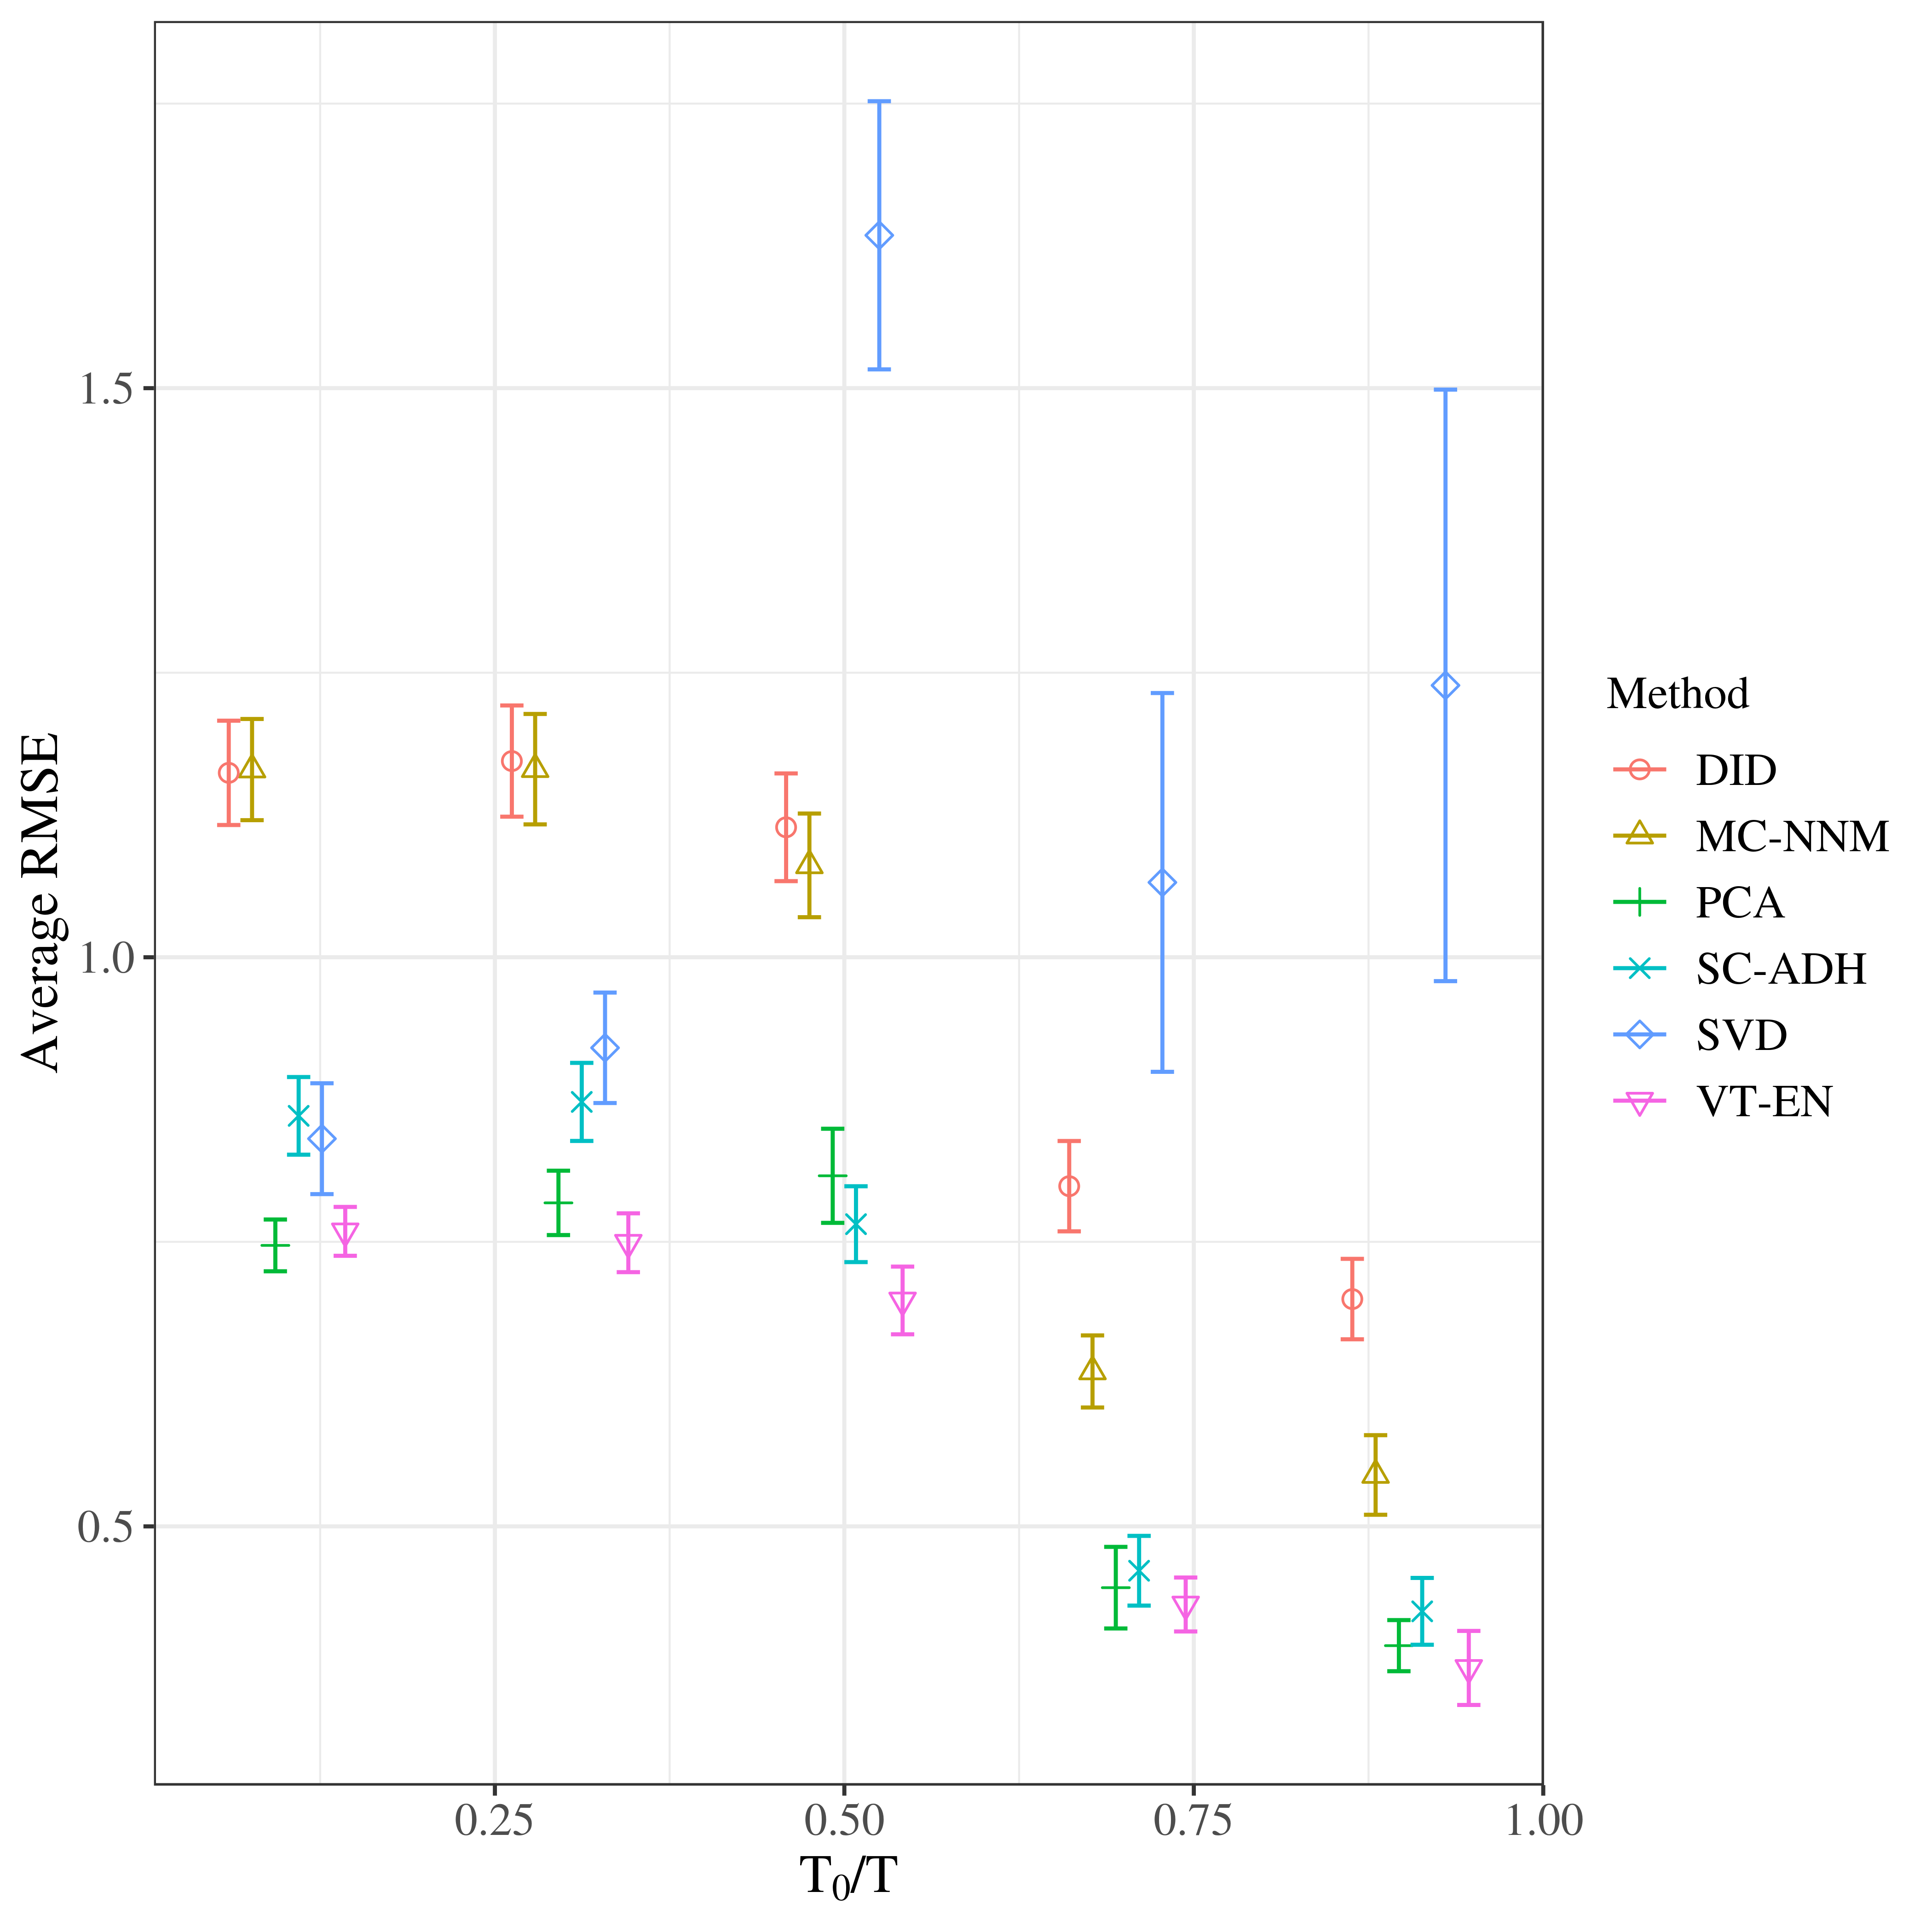
\includegraphics[width=\textwidth]{plots/rev_pc_N_18_T_158_numruns_20_num_treated_9_simultaneuous_1.png}
		\caption{Revenues, simultaneous adoption}
	\end{subfigure}
	~ 
	\begin{subfigure}[t]{0.48\textwidth}
	\centering
	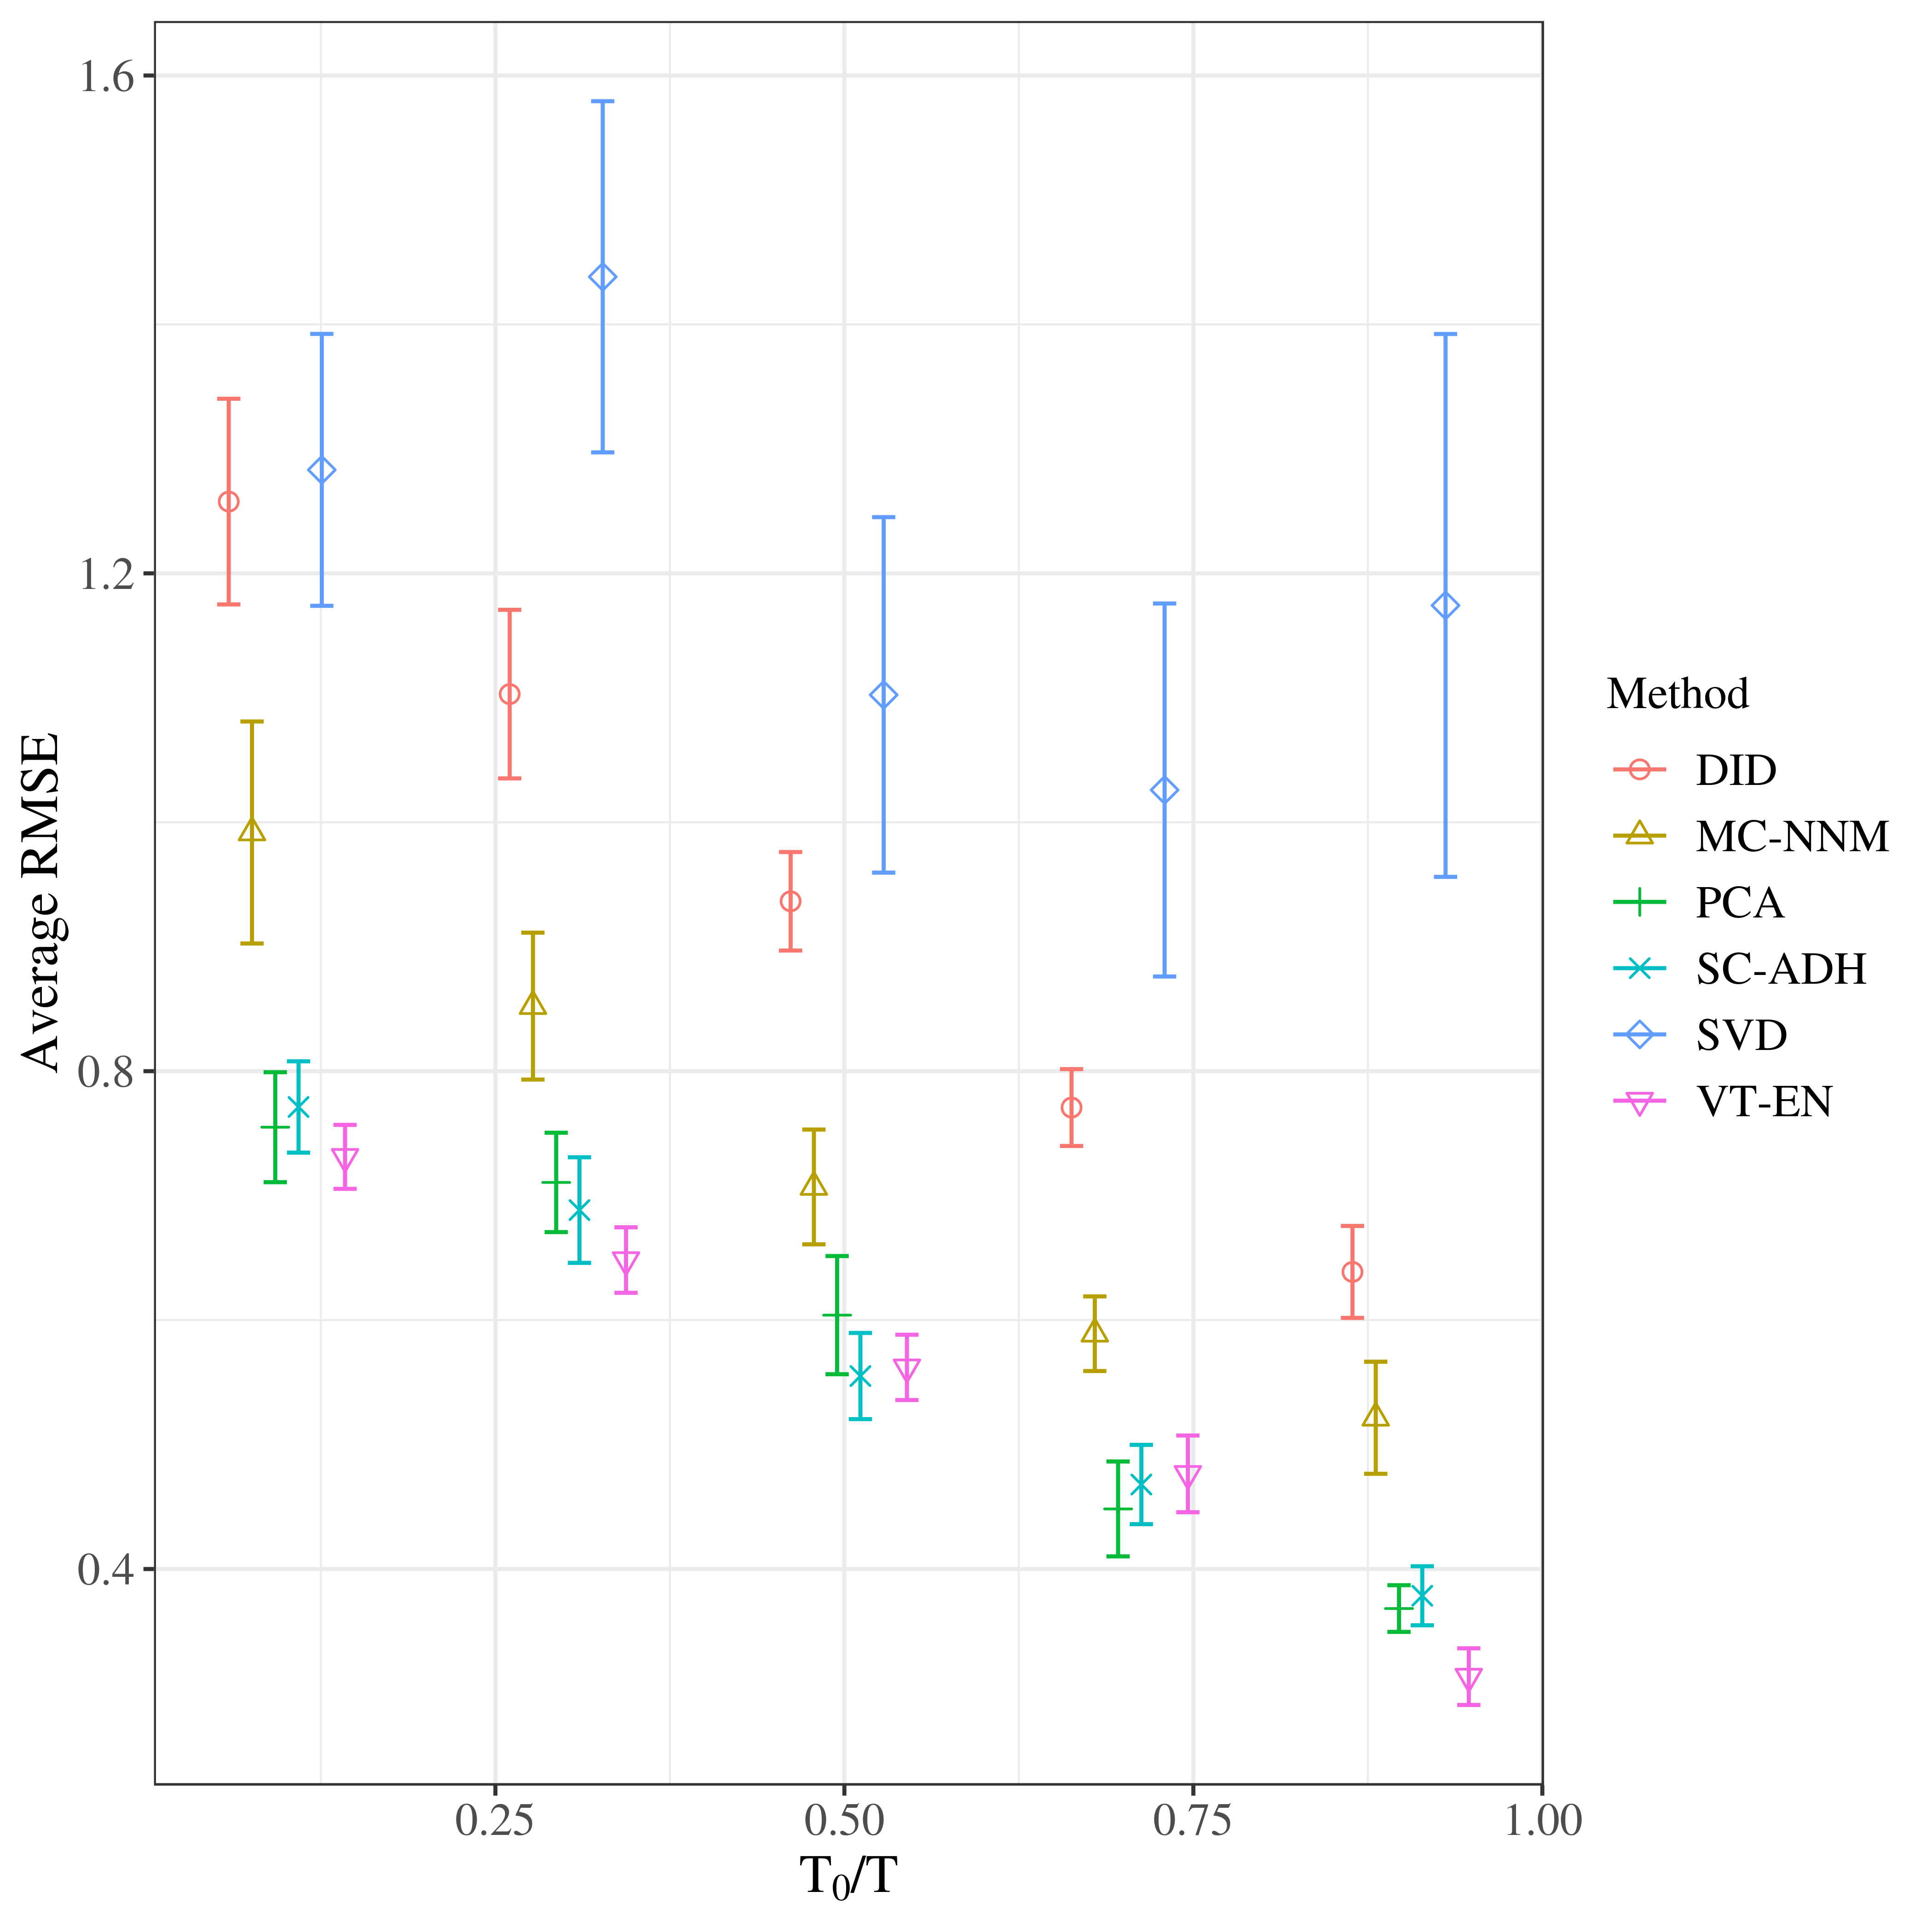
\includegraphics[width=\textwidth]{plots/exp_pc_N_17_T_159_numruns_20_num_treated_9_simultaneuous_0.png}
	\caption{Expenditures, staggered adoption}
\end{subfigure}
~ 
\begin{subfigure}[t]{0.48\textwidth}
	\centering
	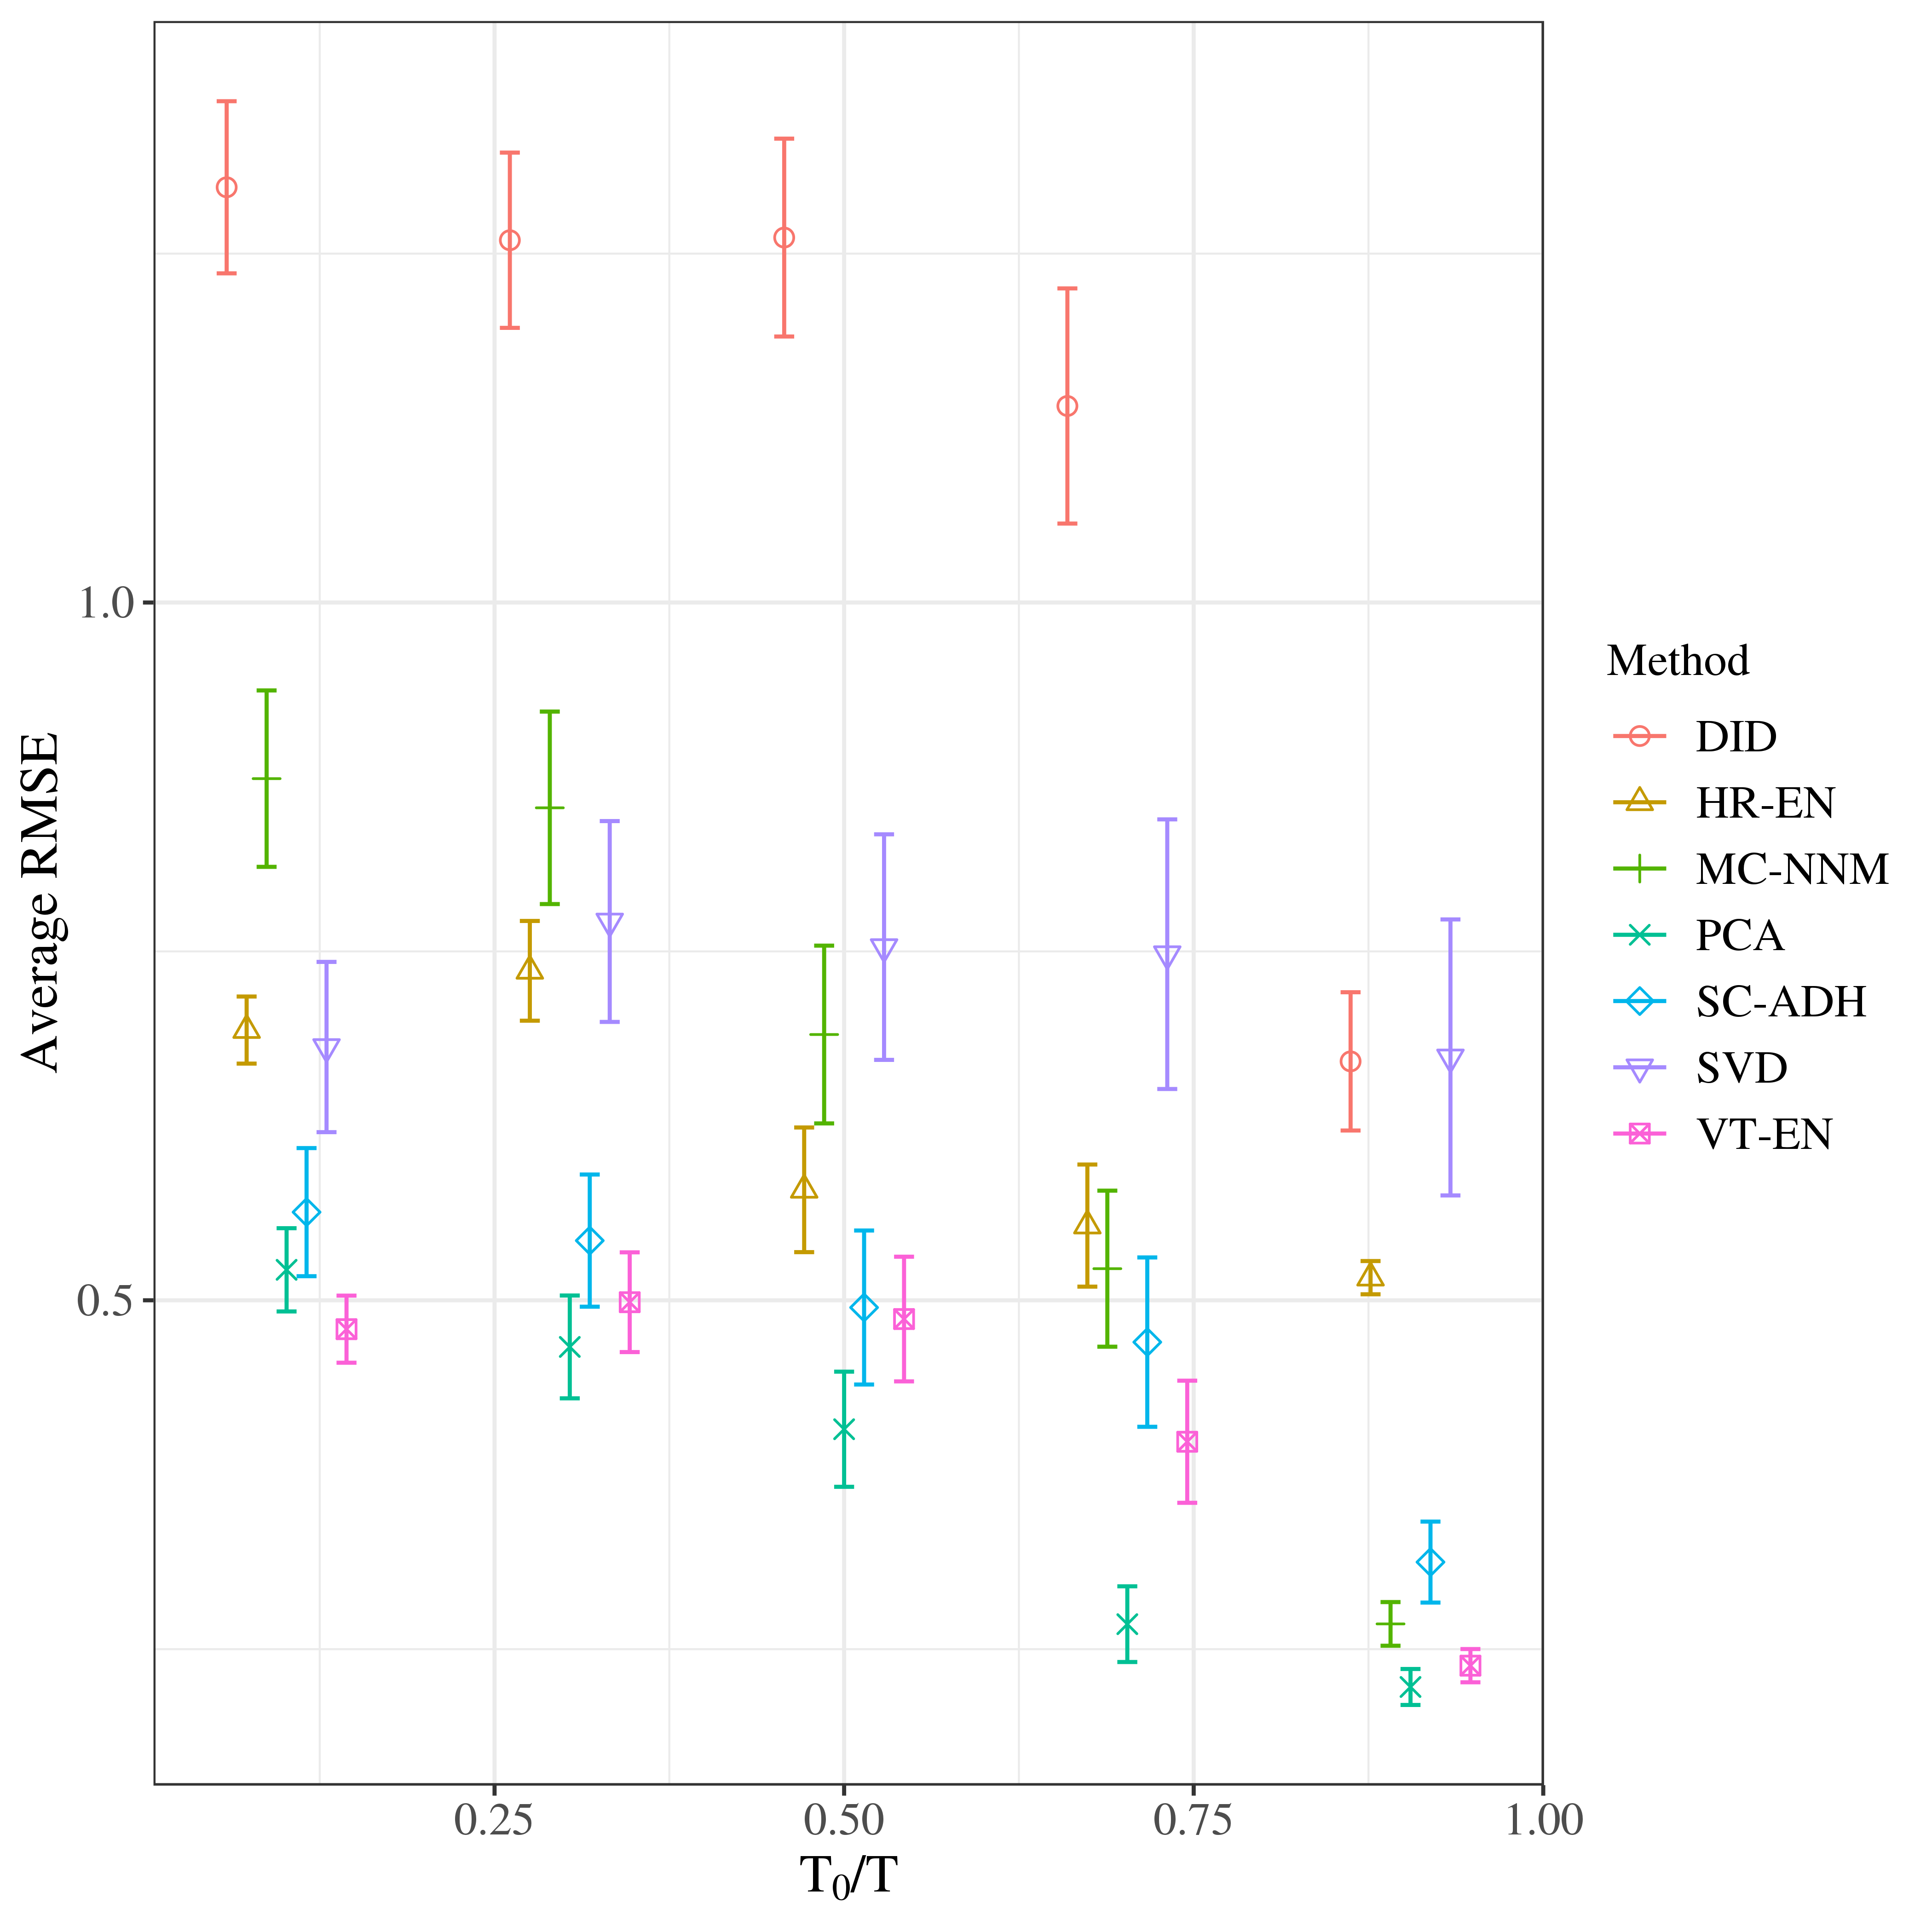
\includegraphics[width=\textwidth]{plots/rev_pc_N_19_T_158_numruns_20_num_treated_10_simultaneuous_0.png}
	\caption{Revenues, staggered adoption}
\end{subfigure}
	\caption{Placebo tests under simultaneous and staggered treatment adoption, with $N_t = 9$. See footnotes to Fig. \ref{synth-sim}. \label{mc-sim}} 
\end{figure}

\pagebreak
\section{Causal mechanisms}

\begin{figure}[htbp]
	\begin{center}
		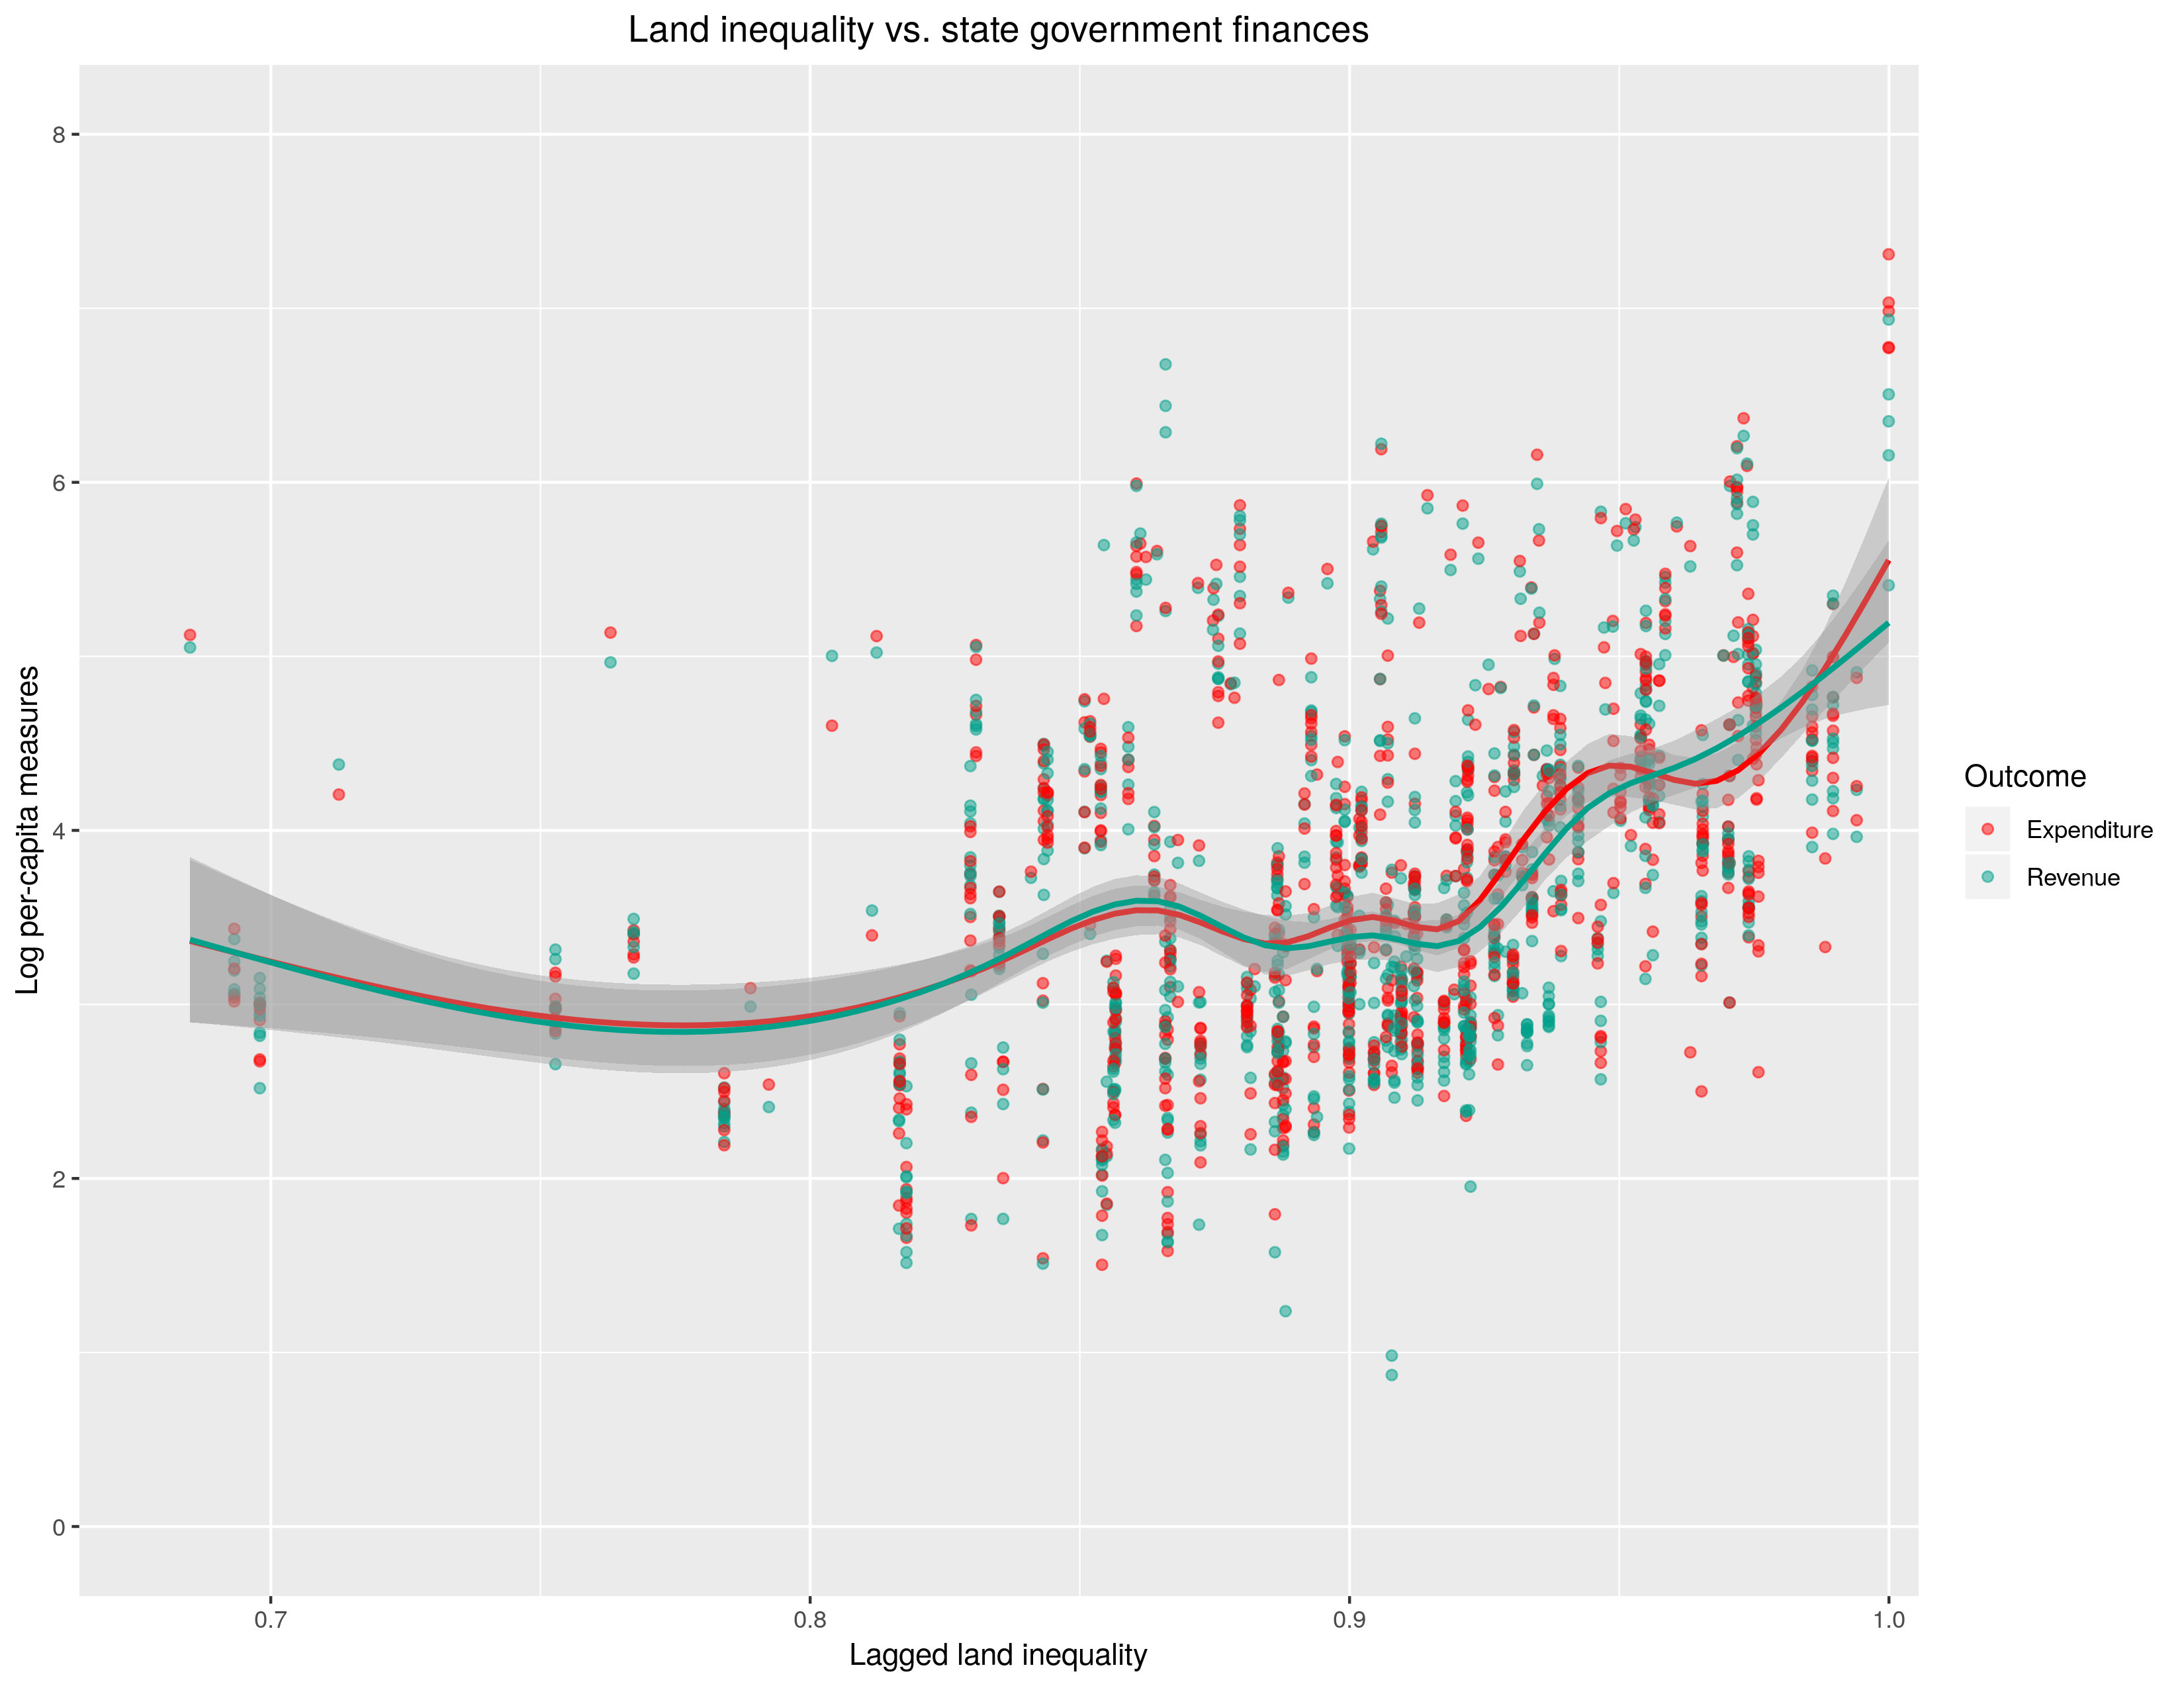
\includegraphics[width=1\textwidth]{plots/ineq-capacity.png} 
	\end{center}
	\caption{Land inequality (lagged by 10 years) vs. log per-capita revenue and expenditure, 1860-1950. Each point is a state-year observation. Lines represent generalized additive model (GAM) fits to the data and shaded regions represent corresponding 95\% confidence intervals.   \label{fig:ineq-capacity}}
\end{figure} 

\pagebreak

%Bibliography
\bibliographystyle{chicago}
\bibliography{references}
%\begin{thebibliography}{}
%\end{thebibliography}


\itemize
\end{document}
